%**************************************************************************************
% License:
% CC BY-NC-SA 4.0 (http://creativecommons.org/licenses/by-nc-sa/4.0/)
%**************************************************************************************

\documentclass[notes]{beamer}

\mode<presentation> {

\usetheme{Madrid}

% Burnt orange
\definecolor{burntorange}{rgb}{0.8, 0.33, 0.0}
\colorlet{beamer@blendedblue}{burntorange}
% Pale yellow
\definecolor{paleyellow}{rgb}{1.0, 1.0, 0.953}
\setbeamercolor{background canvas}{bg=paleyellow}
% Secondary and tertiary palett
\setbeamercolor*{palette secondary}{use=structure,fg=white,bg=burntorange!80!black}
\setbeamercolor*{palette tertiary}{use=structure,fg=white,bg=burntorange!60!black}

% To remove the footer line in all slides uncomment this line
%\setbeamertemplate{footline}
% To replace the footer line in all slides with a simple slide count uncomment this line
%\setbeamertemplate{footline}[page number]

% To remove the navigation symbols from the bottom of all slides uncomment this line
%\setbeamertemplate{navigation symbols}{}
}

\usepackage{amsmath}
\usepackage{bm}
\usepackage{breqn}
\usepackage{graphicx} % for figures
\usepackage{subcaption} % for subplots 
\usepackage[labelsep=space,tableposition=top]{caption}
\renewcommand{\figurename}{Fig.} 
\usepackage{cleveref}
\usepackage{caption,subcaption}% http://ctan.org/pkg/{caption,subcaption}
\usepackage{booktabs} % Allows the use of \toprule, \midrule and \bottomrule in tables
\usepackage{multirow}

% To print 2 slides on a page
%\usepackage{handoutWithNotes}
%\pgfpagesuselayout{2 on 1}[border shrink=2mm]
%----------------------------------------------------------------------------------------
%	TITLE PAGE
%----------------------------------------------------------------------------------------
% The short title appears at the bottom of every slide, the full title is only on the title page
\title[CE394M: Continuum mechanics]{CE394M: An introduction to continuum mechanics} 
\author{Krishna Kumar} % name
\institute[UT Austin] % institution 
{
University of Texas at Austin \\
\medskip
\textit{
  \url{krishnak@utexas.edu}} % Your email address
}
\date{} % Date, can be changed to a custom date

\begin{document}

\begin{frame}
\titlepage % title page as the first slide
\end{frame}
%
%\begin{frame}
% % Table of contents slide, comment this block out to remove it
% \frametitle{Overview}
%  %Throughout your presentation, if you choose to use \section{} and \subsection{} 
%  %commands, these %will automatically be printed on this slide as an overview 
% \tableofcontents
%\end{frame}

\section{Definition of stress and strain tensors}


%----------------------------------------------------------------------------------------
\begin{frame}
\frametitle{Stress vector on a plane}
\begin{figure}[ht]
	\centering
	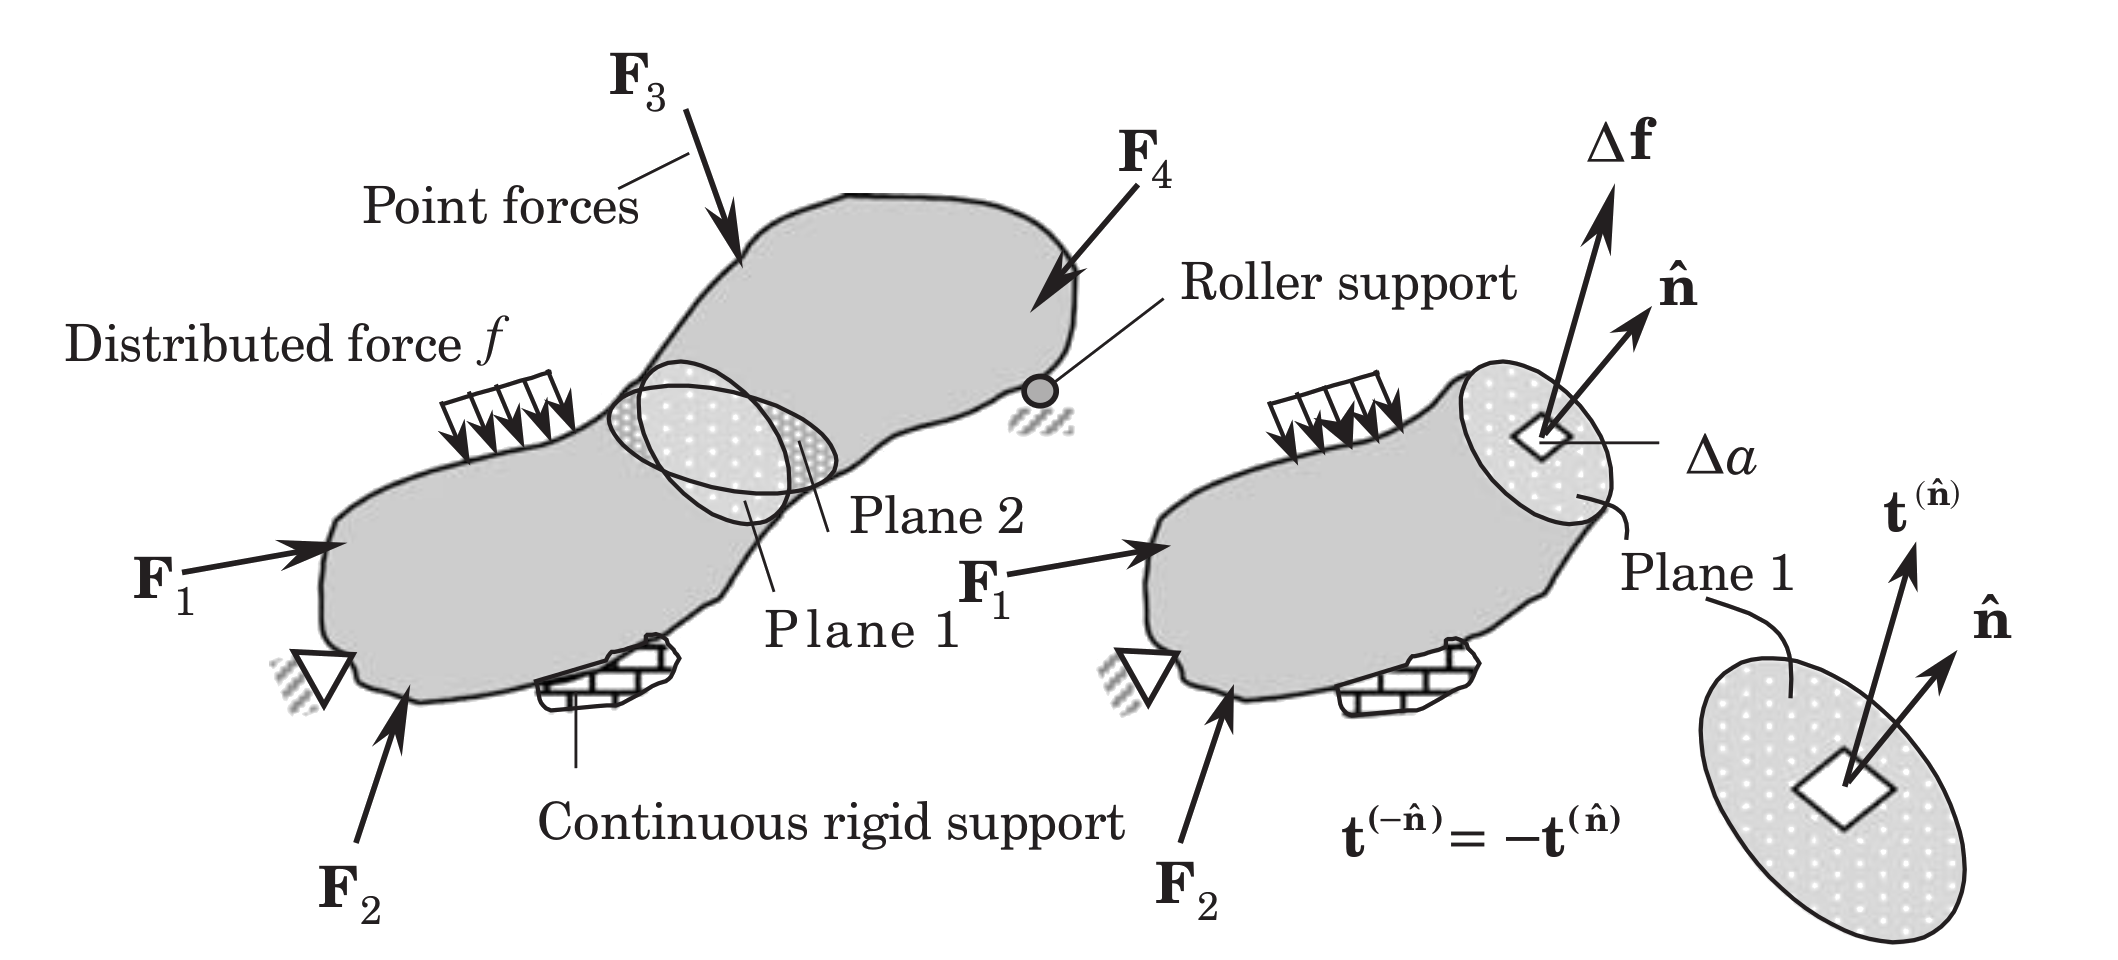
\includegraphics[width=0.7\textwidth]{figs/stress-vector-plane.png}
	\caption*{Stress vector on a plane normal to $\mathbf{\hat{n}}$ (Reddy., 2008)}
\end{figure}

If we denote by $\Delta \mathbf{f(\hat{n})}$ the force on a small area $\mathbf{\hat{n}}$ located at the position $x$, the stress vector can be defined:
\mode<beamer>{	
	\begin{equation*}
		\mathbf{t(\hat{n})} = \lim_{\Delta a \to 0} \frac{\Delta \mathbf{f(\hat{n})}}{\Delta a}
	\end{equation*}
Cauchy stress is the true stress, that is, stress in the deformed configuration.
}
\mode<handout>{	
	\vspace{2cm}
}
\end{frame}

%----------------------------------------------------------------------------------------
\begin{frame}
	\frametitle{Stress vector on a plane}
	\begin{figure}
		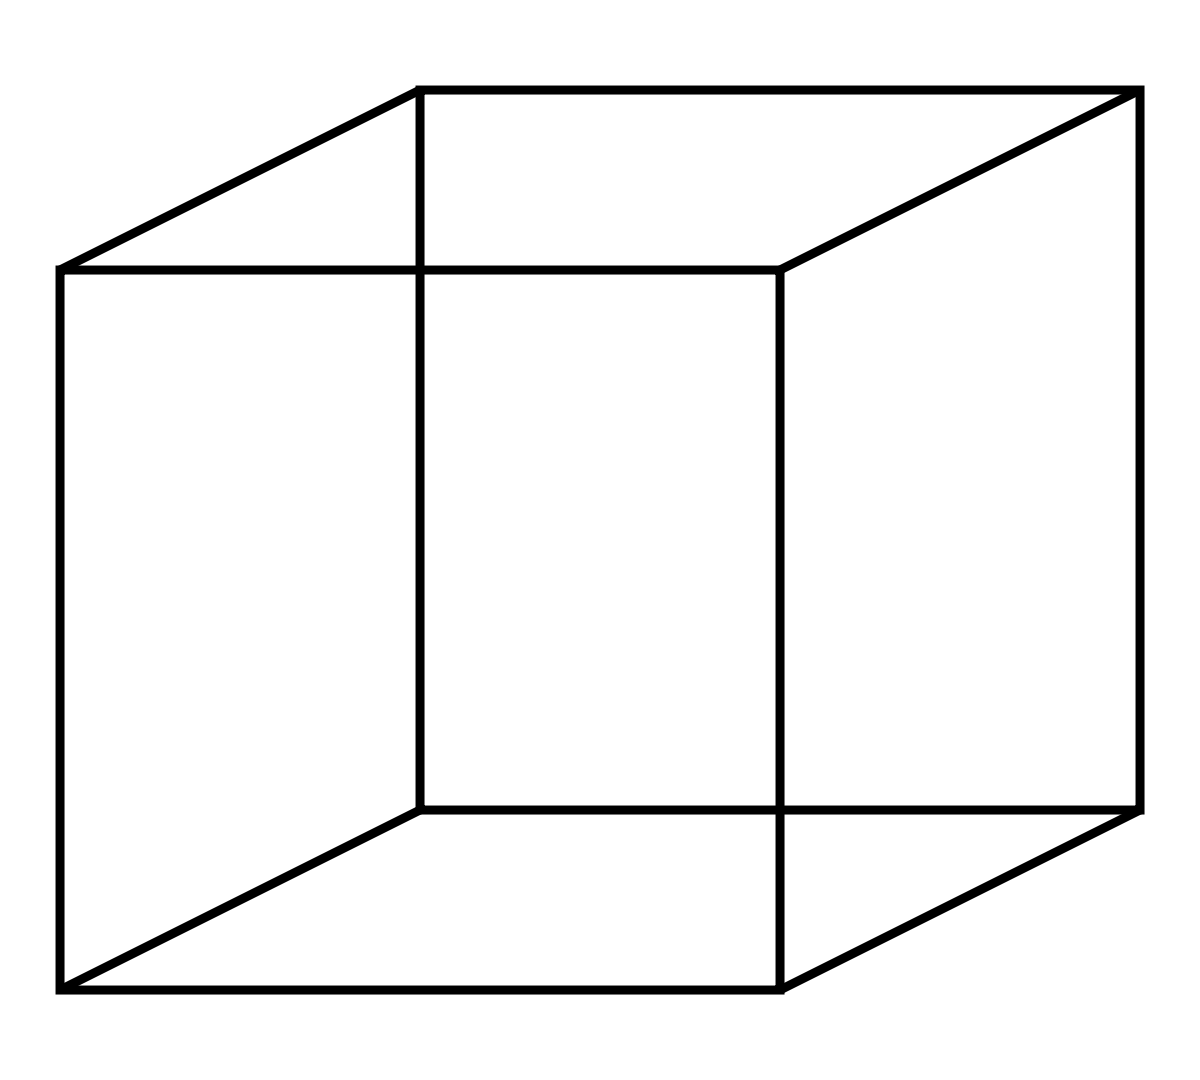
\includegraphics[width=0.5\textwidth]{figs/cube.png}
	\end{figure}
\end{frame}
%----------------------------------------------------------------------------------------
\begin{frame}
\frametitle{Cauchy stress theorem}
The stress vector in the direction of $\mathbf{\hat{n}}$ is:
\mode<beamer>{	
	\begin{equation*}
	\mathbf{t}(\mathbf{\hat{n}}) = 
	 \sigma^T \cdot \mathbf{\hat{n}}
	\end{equation*}

The stress vector $\mathbf{t}$ represents the vectorial stress on a plane whose normal is $\mathbf{\hat{n}}$. $\sigma$ is the \textit{Cauchy stress tensor} defined to be the \textit{current force per unit deformed area}. In Cartesian component, the Cauchy formula is: $t_i = n_j\sigma_{ji}$.

The Cauchy stress tensor $\sigma$, which takes a directional unit vector $e$ as input and maps it to the stress vector $t(e)$, which is the force per unit area.
}
\mode<handout>{
	\vspace{4cm}
}

\begin{figure}[ht]
	\centering
	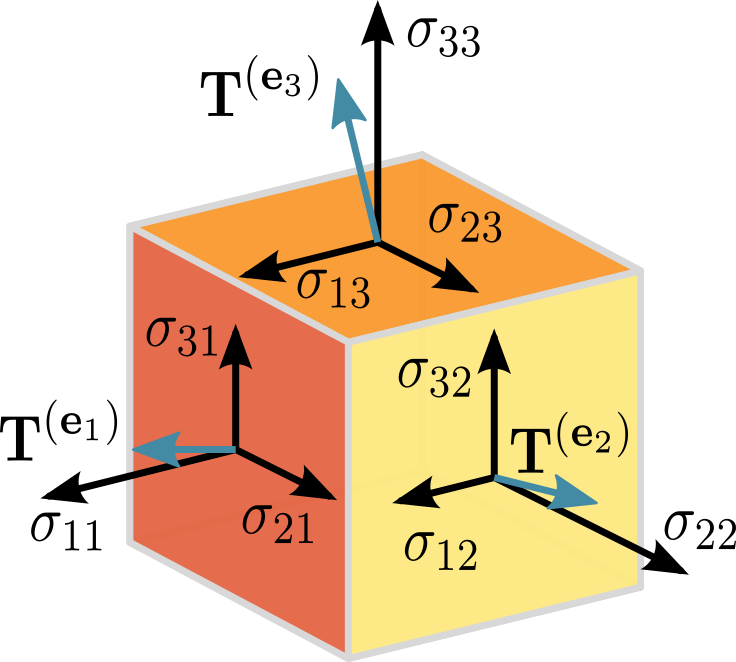
\includegraphics[width=0.3\textwidth]{figs/cauchy-stress.png}
\end{figure}
\end{frame}


%----------------------------------------------------------------------------------------
\begin{frame}
	\frametitle{Cauchy Stress theorem}
	The stress vector $\mathbf{t}$ is now written as a 3-component column vector. The equation tells how to write three equations for the components of $\mathbf{t}$, by multiplying the stress matrix by the unit vector $\mathbf{n}$.
	\begin{equation*}
	\begin{bmatrix}
	t_1 \\
	t_2 \\
	t_3 \\
	\end{bmatrix} = %
	\begin{bmatrix}
	\sigma_{11} & \sigma_{12} & \sigma_{13}\\
	\sigma_{21} & \sigma_{22} & \sigma_{23} \\
	\sigma_{31} & \sigma_{32} & \sigma_{33} \\
	\end{bmatrix} %
	\begin{bmatrix}
	n_1 \\
	n_2 \\
	n_3 \\
	\end{bmatrix}
	\end{equation*}
	
	
	
	\begin{align*}
	t_1 & = 	\sigma_{11} n_1 + \sigma_{12} n_2 +  \sigma_{13} n_3 \\
	t_2 & = 	\sigma_{21} n_1 + \sigma_{22} n_2 +  \sigma_{23} n_3 \\
	t_3 & = 	\sigma_{31} n_1 + \sigma_{32} n_2 +  \sigma_{33} n_3 
	\end{align*}
	
	\mode<beamer>{
		Each component of the stress vector $\mathbf{t}$ depends on three components of the stress tensor, and on the three components of the surface normal vector $\mathbf{n}$. Recall that $\mathbf{t}$ is the force applied at each point on the surface of a chosen region of the body by the surrounding material, and that $\mathbf{n}$ is the unit vector normal to that surface at the same point.
	}
\end{frame}

%----------------------------------------------------------------------------------------
\begin{frame}
	\frametitle{Stress tensor}
	\mode<beamer>{	
	\noindent
	\fboxsep=0pt
	\noindent
	\begin{minipage}[t]{0.59\linewidth}
			\begin{itemize}
				\item Stress state at a point is defined by $\sigma_{ij}$ in a frame of reference. 
				\item 9 components of the stresses in 3D.
				\item 6 stresses: $\sigma_{11}, \sigma_{22}, \sigma_{33}, \tau_{12}, \tau_{23}, \tau_{31}$.
				\item Equilibrium of moments require $\tau_{21} = -\tau_{12}, \tau_{32} = - \tau_{23}, \tau_{13} = - \tau_{31}$
				\item Compression is positive
				\item Shear stress, anti-clockwise is positive
				\item In order to write the components in a more concise way we can use the indices notation: $\sigma_{ij}$ (use $i = 1,2,3$ and $j = 1,2,3$)
				\item Correspondence from $x, y, z$ to $1, 2, 3$ (e.g., $\sigma_{11} = \sigma_{xx}, \sigma_{12} = \sigma_{xy}$)
			\end{itemize}
	\end{minipage}%
	\hfill%
	\begin{minipage}[t]{0.39\linewidth}
		\begin{figure}
			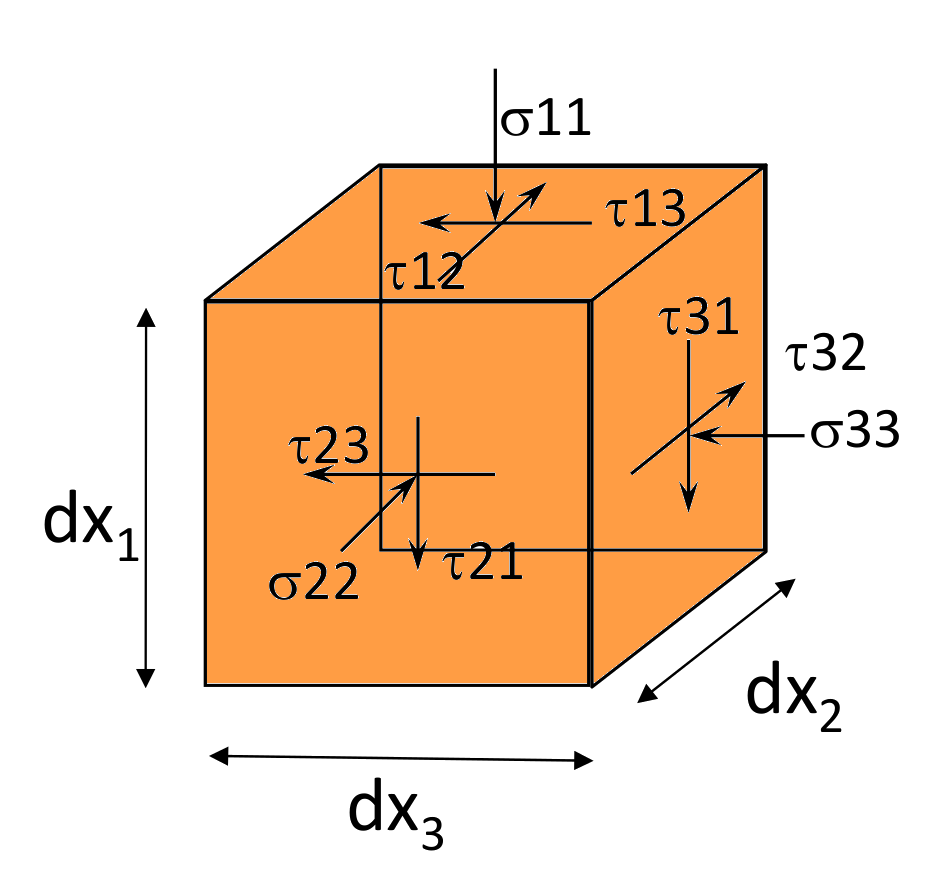
\includegraphics[width=\textwidth]{figs/stresses.png}
		\end{figure}
	\end{minipage}	
	}
	\mode<handout>{
			
		\begin{align*}
		\begin{bmatrix}
		\sigma_{11} & \sigma_{12} & \sigma_{13}\\
		\sigma_{21} & \sigma_{22} & \sigma_{23} \\
		\sigma_{31} & \sigma_{32} & \sigma_{33} \\
		\end{bmatrix}		
		\end{align*}
		
		\begin{figure}
			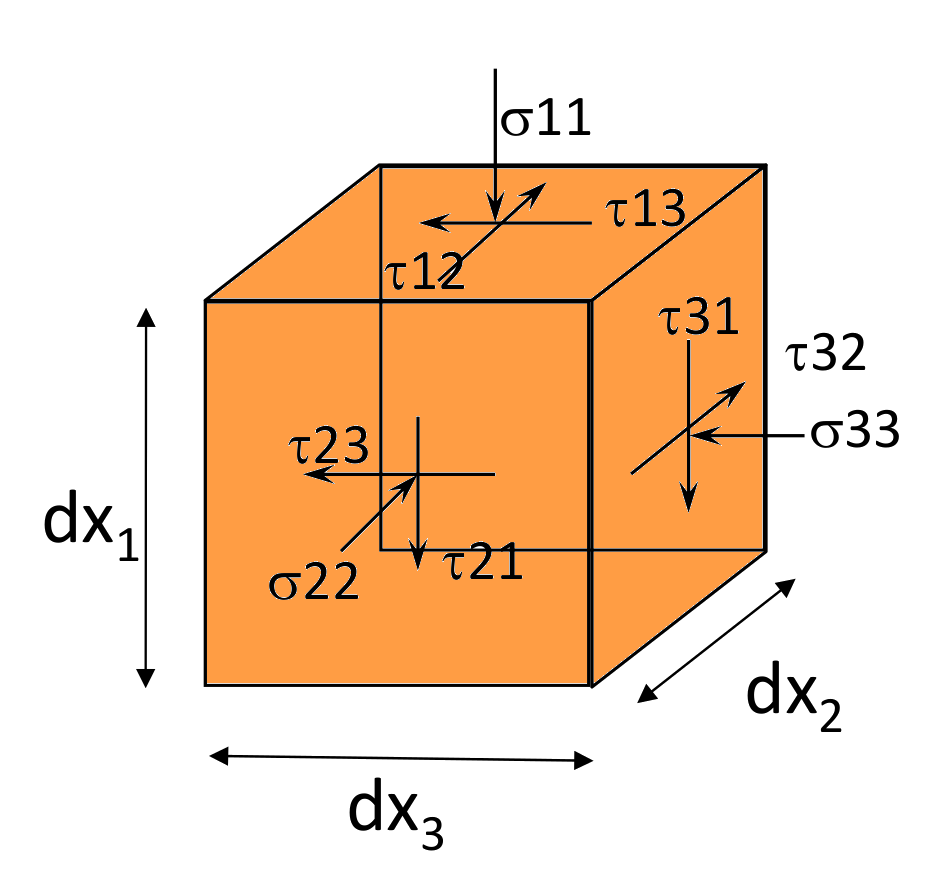
\includegraphics[width=0.5\textwidth]{figs/stresses.png}
		\end{figure}

	}
\end{frame}

%----------------------------------------------------------------------------------------
\begin{frame}
	\frametitle{What is a Tensor?}
	\mode<beamer>{
		\begin{itemize}
			\item A tensor is a geometric object that maps in a multi-linear manner geometric vectors, scalars, and other tensors to a resulting tensor. Vectors and scalars which are often used in elementary physics and engineering applications, are considered as the simplest tensors.
			\item Tensors, defined mathematically, are simply arrays of numbers, or functions, that transform according to certain rules under a change of coordinates. Tensors characterize the properties of a physical system.
			\item An elementary example of mapping, describable as a tensor, is the dot product, which maps two vectors to a scalar. 
			\item A tensor may consist of a single number, in which case it is referred to as a tensor of order zero, or simply a scalar. An example of a scalar field would be the density of a fluid as a function of position.
			\item A second-order tensor is a vector.
		\end{itemize}
	}
\end{frame}


%----------------------------------------------------------------------------------------
\note{
	Assuming a basis of a real vector space, e.g., a coordinate frame in the ambient space, a tensor can be represented as an organized multidimensional array of numerical values with respect to this specific basis. Changing the basis transforms the values in the array in a characteristic way that allows to define tensors as objects adhering to this transformational behavior. For example, there are invariants of tensors that must be preserved under any change of the basis, thereby making only certain multidimensional arrays of numbers a tensor. Compare this to the array representing $\varepsilon _{ijk}$ not being a tensor, for the sign change under transformations changing the orientation.
}

\note{		
	A tensor is often thought of as a generalized matrix. That is, it could be a 1-D matrix (a vector is actually such a tensor), a 3-D matrix (something like a cube of numbers), even a 0-D matrix (a single number), or a higher dimensional structure that is harder to visualize. The dimension of the tensor is called its rank. But this description misses the most important property of a tensor! A tensor is a mathematical entity that lives in a structure and interacts with other mathematical entities. If one transforms the other entities in the structure in a regular way, then the tensor must obey a related transformation rule. This “dynamical” property of a tensor is the key that distinguishes it from a mere matrix. Any rank-2 tensor can be represented as a matrix, but not every matrix is really a rank-2 tensor. The numerical values of a tensor’s matrix representation depend on what transformation rules have been applied to the entire system.
}

\note{
	`\textit{a tensor quantity is a physical quantity which has no specified direction but different values in different directions with an associated transformation between different coordinates.}'
	
	Suppose a car has some velocity represented by $(1, 1, 0)$ m/s, that definition is pretty useless, since there is no information about the coordinate system. However, if we define three orthonormal unit vectors and give the velocity in terms of those vectors, then we have all the information we need. A tensor works is just a generalization of the vector concept (in fact a vector is a rank 1 tensor, and even a scalar can be considered a rank 0 tensor!). 
}

\note{
	Suppose I write down a matrix on a piece of paper and tell you that it represents the moment of inertia of some object. Then I tell you to transform it into a more convenient coordinate system, you can't do it! You have no information about the coordinate system that I used when I calculated the matrix. A moment of inertia tensor is basically a matrix where each element is associated with two unit vectors in some given coordinate system. This is all the info you need to transform into other systems, and the mathematics of such transformations is extremely elegant in tensor notation. So, in short, a tensor is basically a "matrix-like" quantity that is independent of any coordinate system, and can be readily expressed in any coordinate system.
	
	\url{https://www.physicsforums.com/threads/what-is-tensor-quantity.345535/}
}

%----------------------------------------------------------------------------------------
\begin{frame}
	\frametitle{Divergence theorem}
	
	The total contact force acting on $V$ is:
	\mode<beamer>{
		\begin{equation*}
		\int_S \mathbf{T} dS = \int_S \sigma^T \hat{n} dS = \int_V \nabla \cdot \sigma^T dV.
		\end{equation*}
	}
	\mode<handout>{
		\vspace{1.5cm}	
	}
	Divergence theorem converts an integral over $S$ into an integral over the volume $V$ enclosed by $S$.
	\begin{figure}
		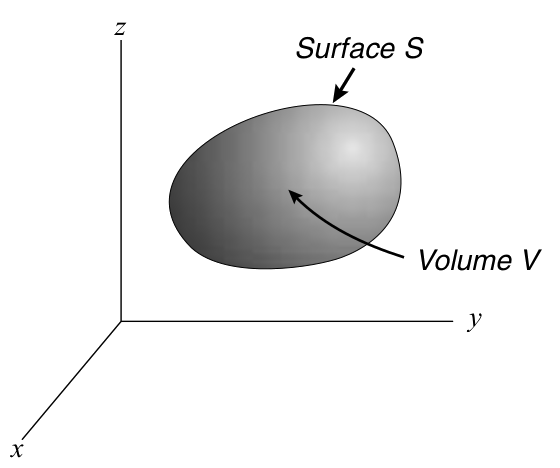
\includegraphics[width=0.5\textwidth]{figs/region-surface-volume.png}
	\end{figure}
\end{frame}

%----------------------------------------------------------------------------------------
\begin{frame}
	\frametitle{Equilibrium}
	
	If we assume that the body is in static equilibrium, we must set the contact forces and body forces equal. 
	
	\mode<beamer>{
		\begin{equation*}
		\int_V \nabla \cdot \sigma^T dV = \int_V \mathbf{b} dV
		\end{equation*}
	}
	\mode<handout>{
		\vspace{1.5cm}	
	}
	\begin{align*}
		\frac{\partial \sigma_{xx}}{\partial x} +%
		\frac{\partial \sigma_{xy}}{\partial y} +%
		\frac{\partial \sigma_{xz}}{\partial z} - b_x &= 0 \\
		%
		\frac{\partial \sigma_{yx}}{\partial x} +%
		\frac{\partial \sigma_{yy}}{\partial y} +%
		\frac{\partial \sigma_{yz}}{\partial z} - b_y &= 0\\
		%
		\frac{\partial \sigma_{zx}}{\partial x} +%
		\frac{\partial \sigma_{zy}}{\partial y} +%
		\frac{\partial \sigma_{zz}}{\partial z} - b_z &= 0 \\
	\end{align*}
\end{frame}


\subsection{Descriptions of Motion}
%----------------------------------------------------------------------------------------
\begin{frame}
\frametitle{Descriptions of Motion}

For a given geometry and loading, the body \textit{B} will undergo macroscopic geometric
changes within the body, which are termed deformation. The geometric changes are
accompanied by stresses that are induced in the body.

\begin{figure}
	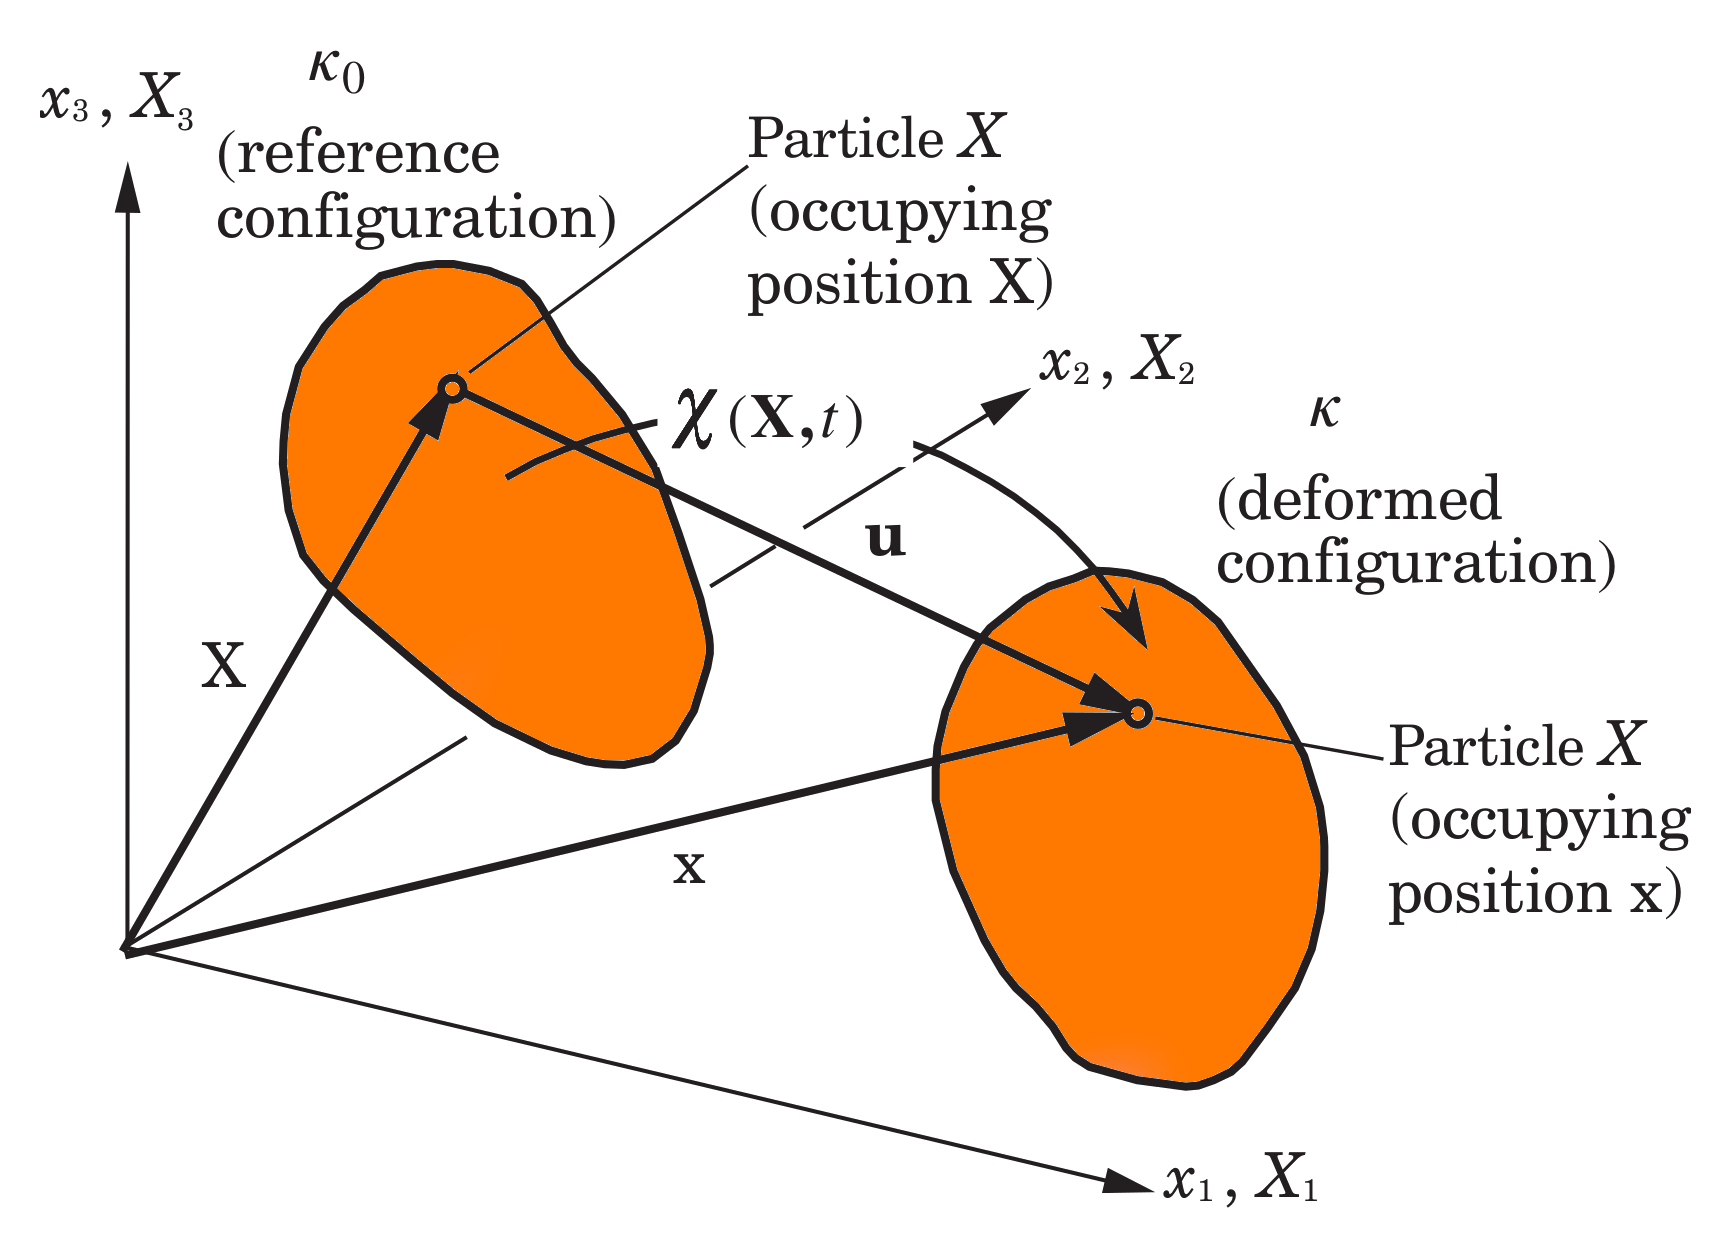
\includegraphics[width=0.65\textwidth]{figs/deformation-body.png}
\end{figure}
\end{frame}

%----------------------------------------------------------------------------------------
\begin{frame}
	\frametitle{Descriptions of Motion: Displacement field}
	The displacement of the particle X is given: $\mathbf{u = x -X}$.
	\noindent
	\fboxsep=0pt
	\noindent
	\begin{minipage}[t]{0.49\linewidth}
		\centering
		\begin{figure}
			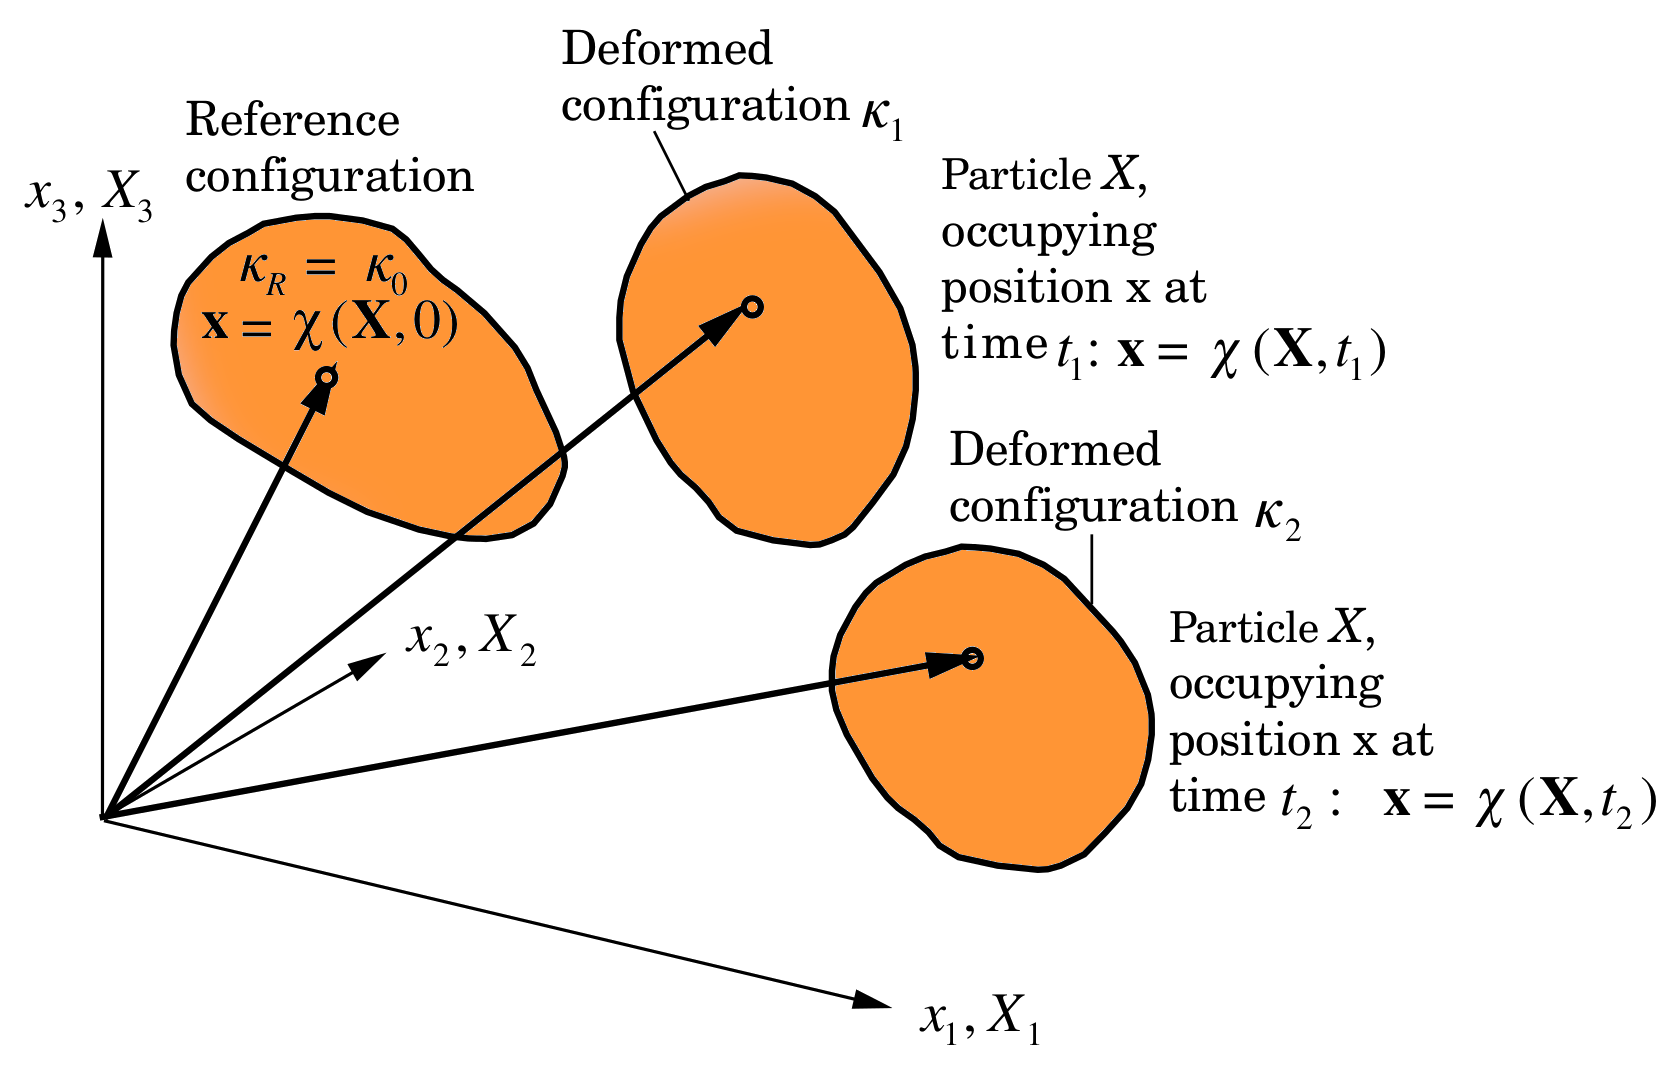
\includegraphics[width=\textwidth]{figs/lagrangian.png}
			\caption*{Lagrangian}
		\end{figure}
		\mode<beamer>{$\mathbf{u}(\mathbf{X}, t) = \mathbf{x}(\mathbf{X}, t) - \mathbf{X}$}
	\end{minipage}%
	\hfill%
	\begin{minipage}[t]{0.49\linewidth}
		\centering
		\begin{figure}
			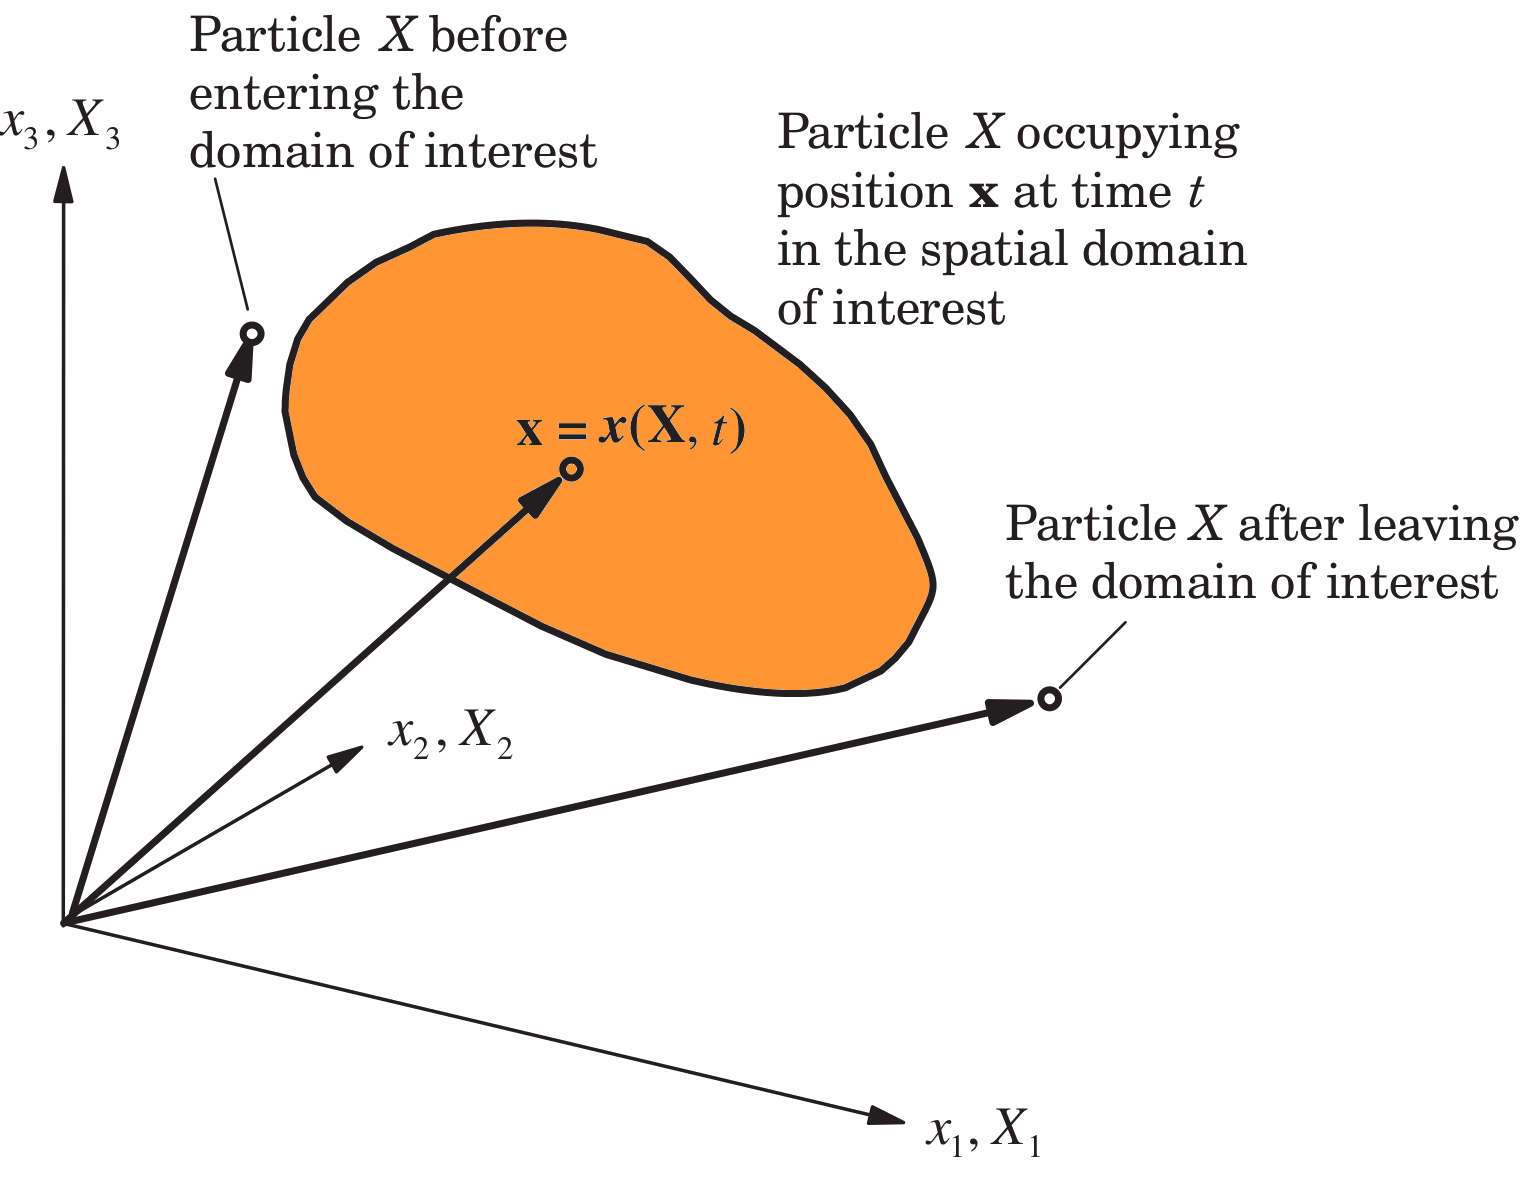
\includegraphics[width=0.8\textwidth]{figs/eulerian.png}
			\caption*{Eulerian}
		\end{figure}
		\mode<beamer>{$\mathbf{u}(\mathbf{x}, t) = \mathbf{x - X}(\mathbf{x}, t)$}
	\end{minipage}	
\end{frame}


\note{
	The mathematical description of the deformation of a continuous body follows
	one of the two approaches: (1) the material description and (2) spatial description.
	The material description is also known as the Lagrangian description, and the spatial
	description is known as the Eulerian description.
	
	In the material description, the motion of the body is referred to a reference 
	configuration $k_R$, which is often chosen to be the undeformed configuration, $k_R = k_0$.
	Thus, in the Lagrangian description, the current coordinates ($x \in k$) are expressed
	in terms of the reference coordinates ($X \in k_0$).
	
	In the spatial description, the motion is referred to the current configuration $k$ 
	occupied by the body $B$, and $\phi$ is described with respect to the current position 
	($x \in k$) in space, currently occupied by material particle $X$.
}

%----------------------------------------------------------------------------------------
\begin{frame}
\frametitle{Deformation Gradient Tensor}

\begin{figure}
	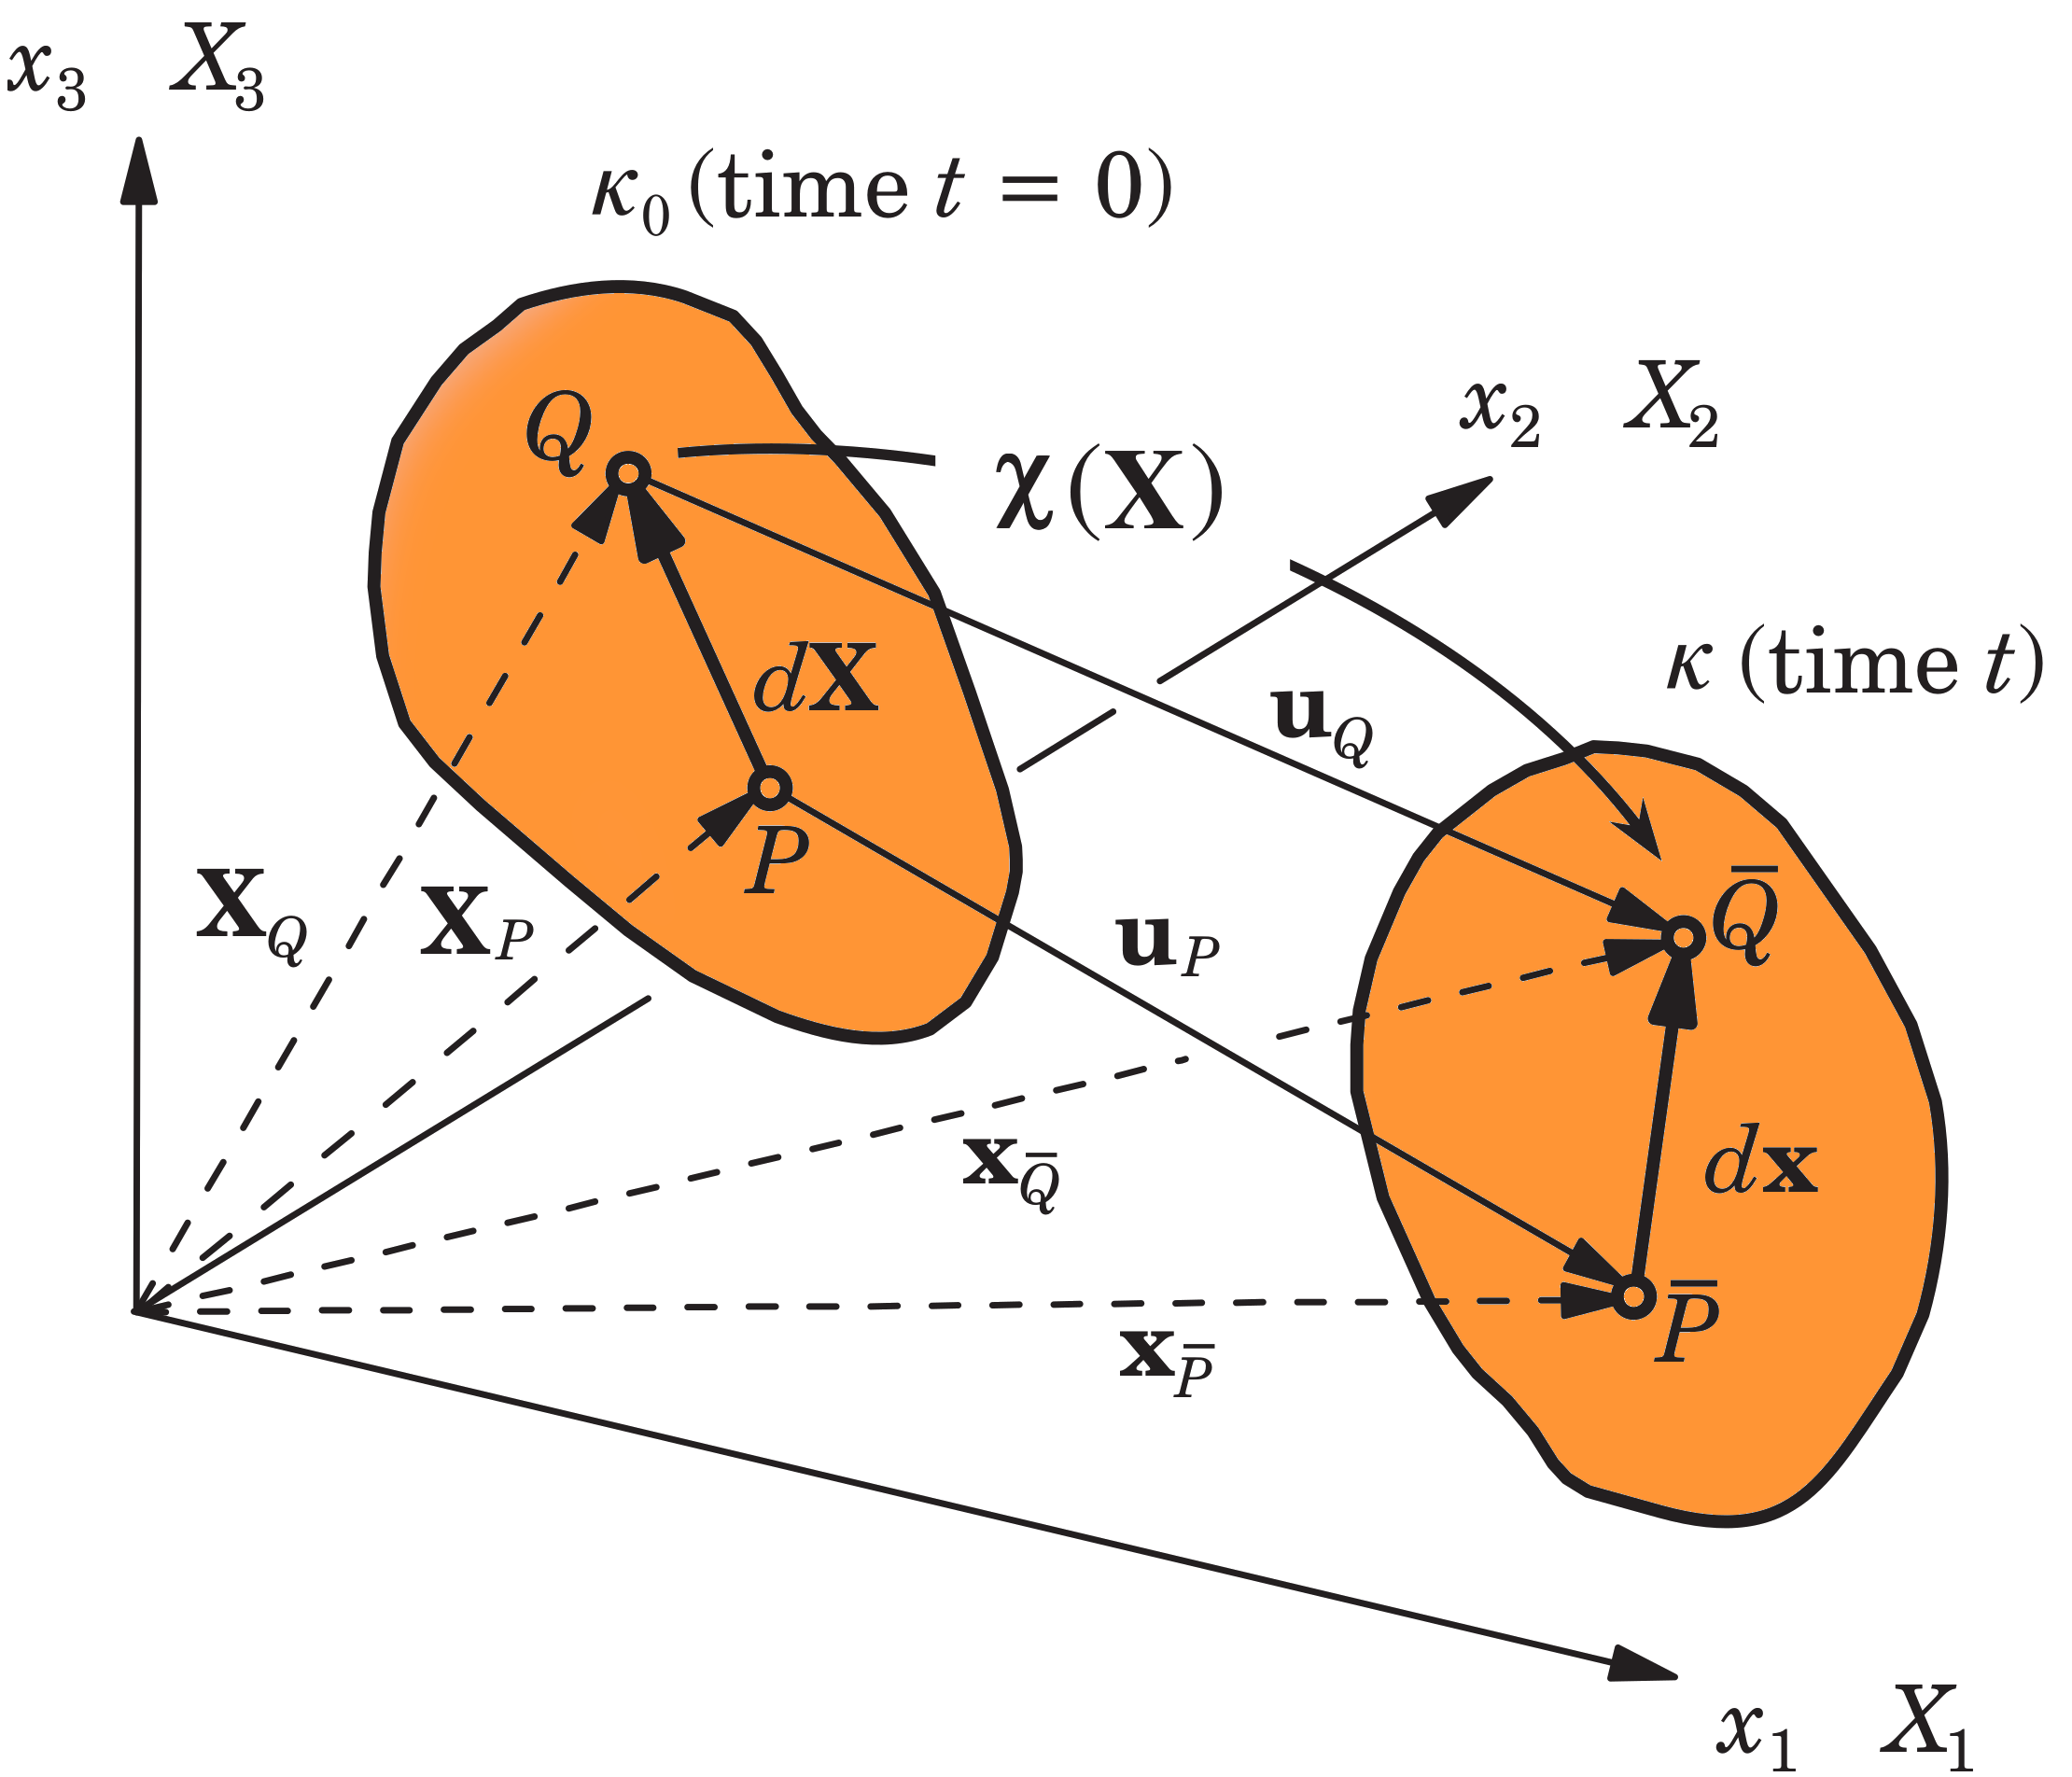
\includegraphics[width=0.6\textwidth]{figs/green-strain.png}
	\caption*{Points $P$ and $Q$ separated by a distance $d\mathbf{X}$ in the undeformed configuration $k_0$ take up positions $\bar{P}$ and $\bar{Q}$, respectively, in the deformed configuration $k$, where they are separated by distance $d\mathbf{x}$}
\end{figure}
\end{frame}

\note{The deformation gradient is a tensor that quantifies both the 3D and 2D shape change as well as overall material rotation, making it superior to strain as an all-encompassing measure of deformation of material elements.}

%----------------------------------------------------------------------------------------
\begin{frame}
\frametitle{Deformation Gradient Tensor}

deformation gradient $F_k$ of $k$ relative to the reference configuration $k_0$, 
which gives the relationship of a material line $dX$ before deformation to the line $dx$ (consisting of the same material as $dX$) after deformation.

\mode<beamer>{
	\begin{align*}
		d\mathbf{x} & = \mathbf{F} \cdot d \mathbf{X} = d \mathbf{X} \cdot \mathbf{F}^T \\
		\mathbf{F} & = \left(\frac{\partial \mathbf{x}}{\partial \mathbf{X}}\right)^T \\
		d\mathbf{X} & = \mathbf{F}^{-1} \cdot d\mathbf{x} = d\mathbf{x} \cdot \mathbf{F}^{-T}
	\end{align*}
}
\mode<handout>{
	\vspace{3cm}
}
\begin{equation*}
	\left[\mathbf{F}\right] = 
	\begin{bmatrix}
		\frac{\partial x_1}{\partial X_1} & \frac{\partial x_1}{\partial X_2} & \frac{\partial x_1}{\partial X_3} \\
		\frac{\partial x_2}{\partial X_1} & \frac{\partial x_2}{\partial X_2} & \frac{\partial x_2}{\partial X_3} \\		\frac{\partial x_3}{\partial X_1} & \frac{\partial x_3}{\partial X_2} & \frac{\partial x_3}{\partial X_3} \\
	\end{bmatrix}
\end{equation*}
\end{frame}


%----------------------------------------------------------------------------------------
\begin{frame}
\frametitle{Deformation Gradient Tensor}

Isotropic compression/extension:
\mode<beamer>{
	\begin{equation*}
		\left[\mathbf{F}\right] = 
		\begin{bmatrix}
			\lambda & 0 & 0 \\
			0 & \lambda & 0 \\
			0 & 0 & \lambda \\
		\end{bmatrix}
	\end{equation*}
	Isochoric (constant volume) is a special case where $\lambda = 1$.
}
\mode<handout>{
	\vspace{2cm}
}
Simple extension:
\mode<beamer>{
	\begin{equation*}
	\left[\mathbf{F}\right] = 
	\begin{bmatrix}
	1 + \alpha & 0 & 0 \\
	0 & 1 & 0 \\
	0 & 0 & 1 \\
	\end{bmatrix}
	\end{equation*}
}
\mode<handout>{
	\vspace{2cm}
}

Simple shear:
\mode<beamer>{
	\begin{equation*}
	\left[\mathbf{F}\right] = 
	\begin{bmatrix}
	1 & \gamma & 0 \\
	0 & 1 & 0 \\
	0 & 0 & 1 \\
	\end{bmatrix}
	\end{equation*}
}
\mode<handout>{
	\vspace{2cm}
}
It is rather difficult to invert the mapping even for this simple nonhomogeneous deformation.
\end{frame}

\subsection{Strain measures}
%----------------------------------------------------------------------------------------
\begin{frame}
\frametitle{Deformation Tensors}

\begin{figure}
	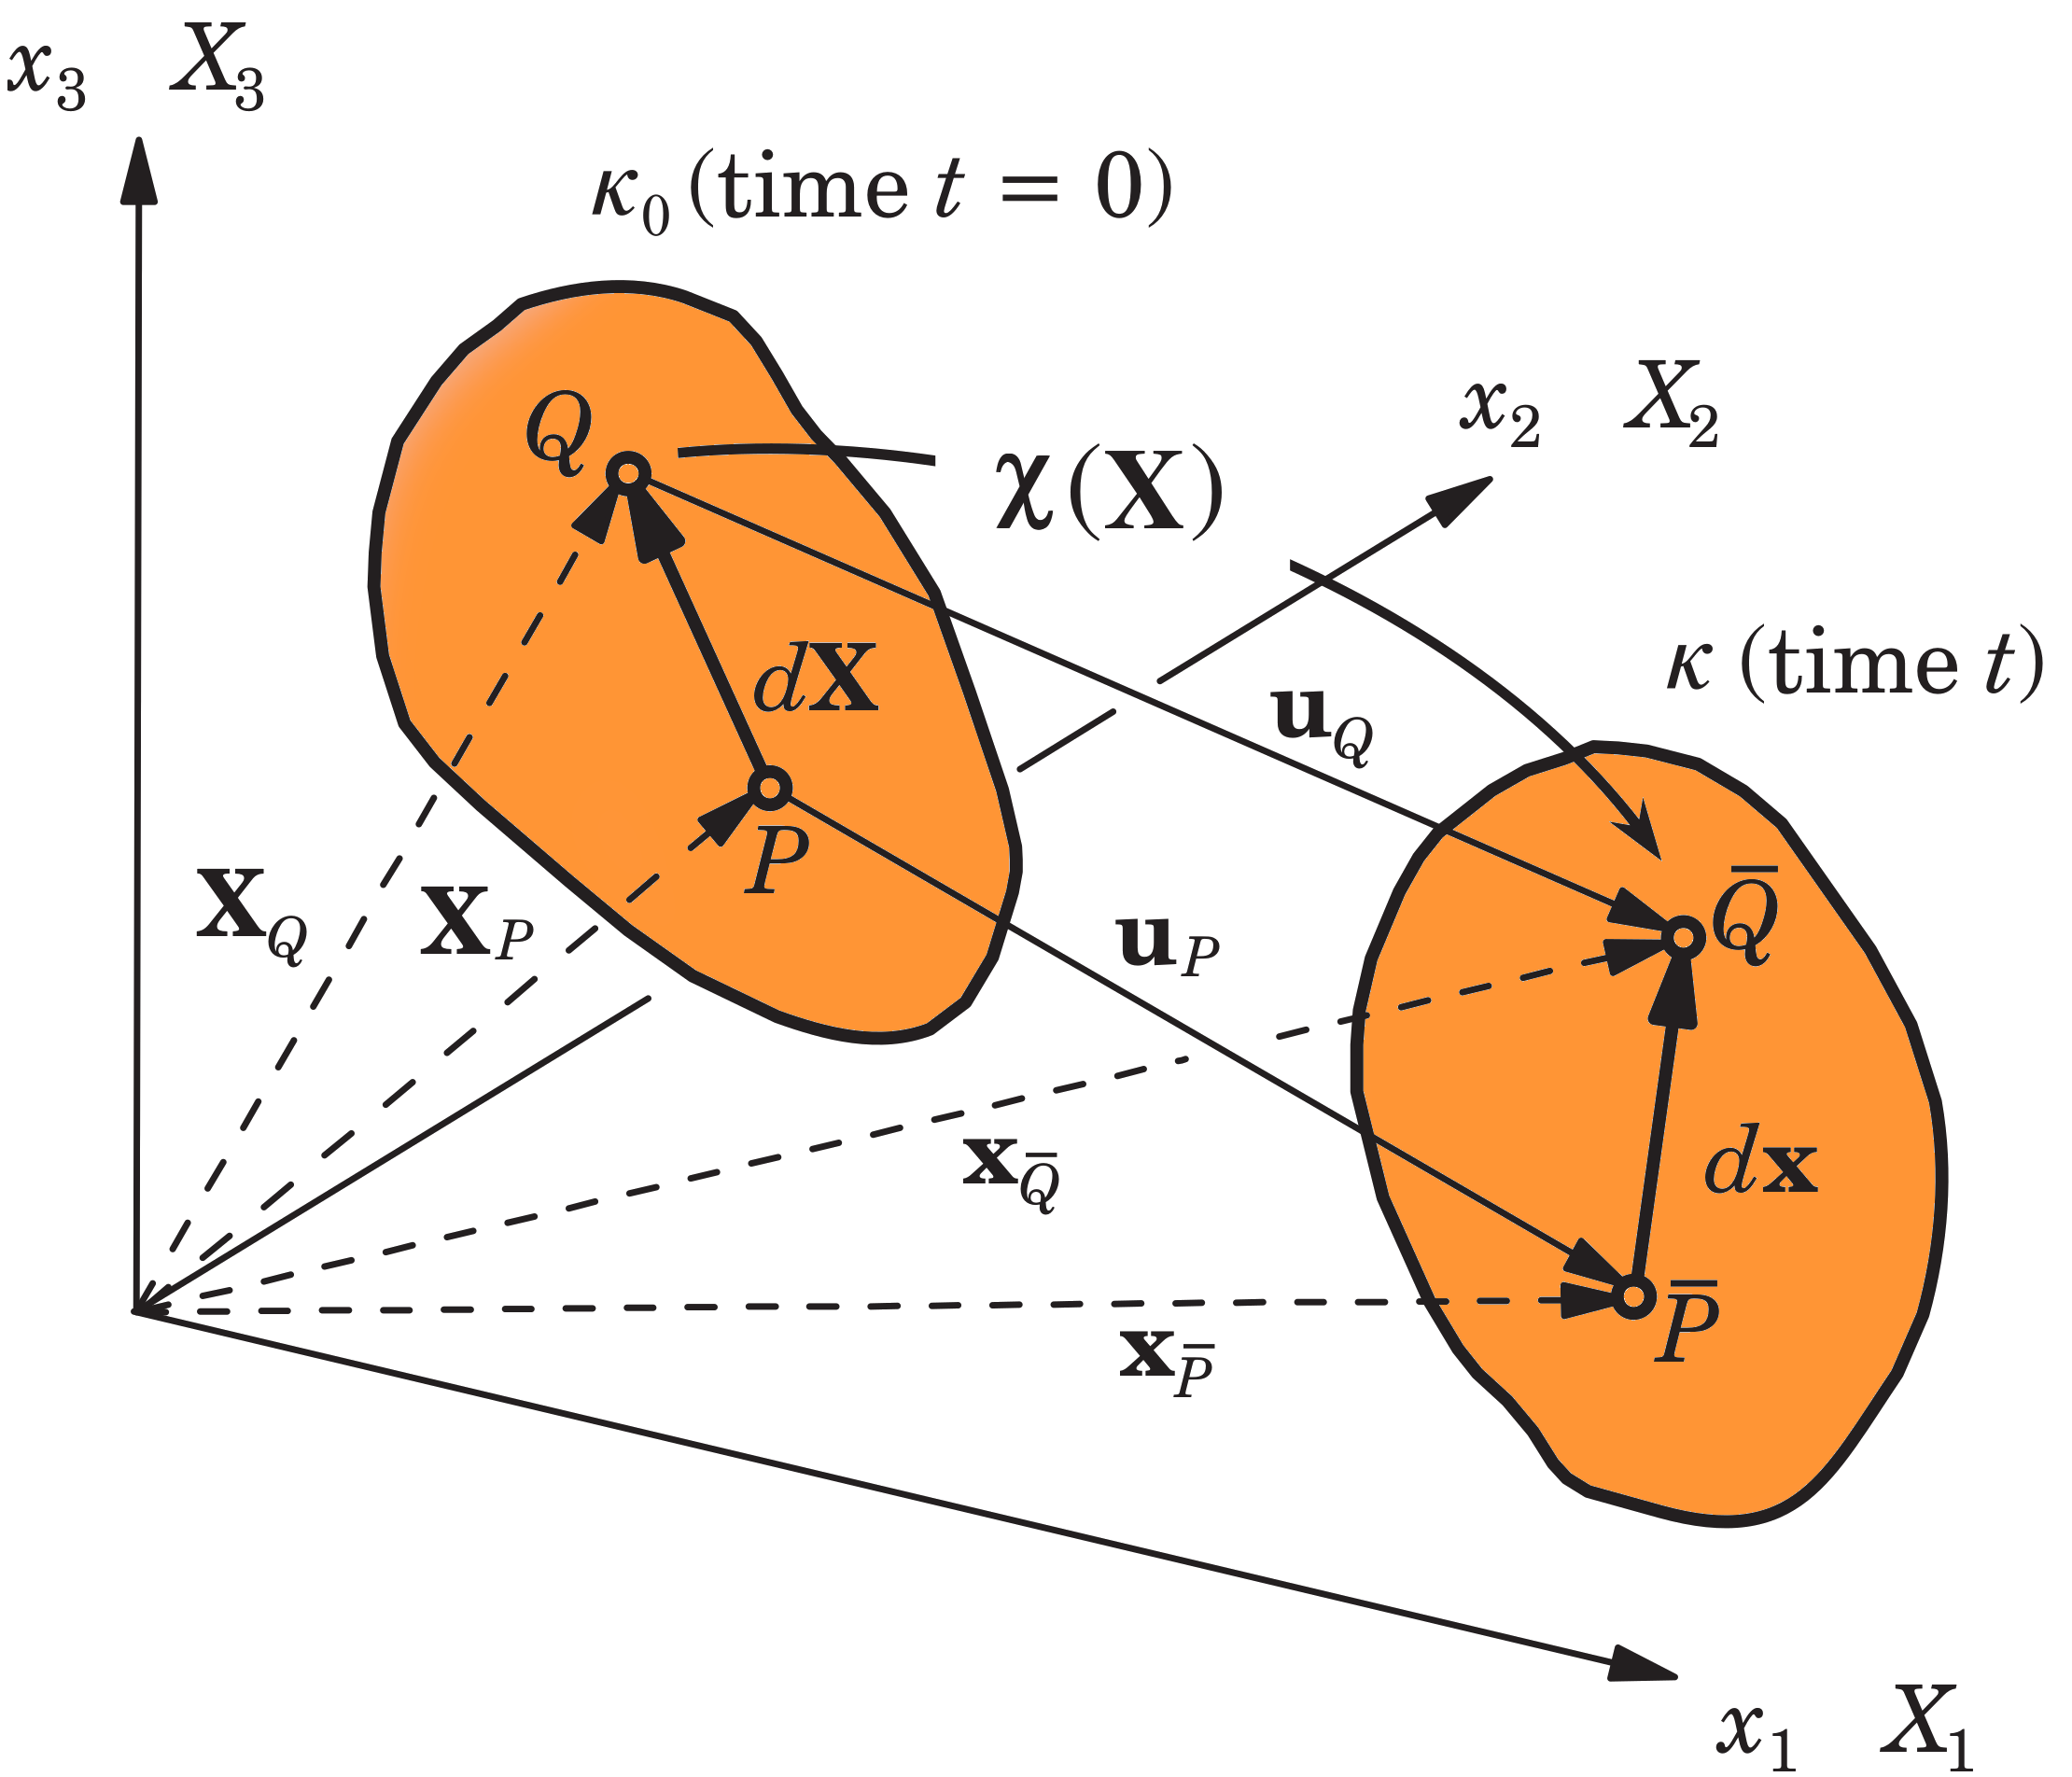
\includegraphics[width=0.6\textwidth]{figs/green-strain.png}
	\caption*{Points $P$ and $Q$ separated by a distance $d\mathbf{X}$ in the undeformed configuration $k_0$ take up positions $\bar{P}$ and $\bar{Q}$, respectively, in the deformed configuration $k$, where they are separated by distance $d\mathbf{x}$}
\end{figure}
\end{frame}

%----------------------------------------------------------------------------------------
\begin{frame}
\frametitle{Eulerian Strain Tensor}

The change in the squared lengths that occurs as a body deforms from the reference to the current configuration can be expressed relative to the original length as:
	\begin{align*}
	(ds)^2  - (dS)^2 & = 2 d\mathbf{x} \cdot \mathbf{e} \cdot d\mathbf{x}, \\
	\varepsilon & = \frac{1}{2}(\mathbf{I} - \mathbf{F}^T \cdot \mathbf{F}^{-1})
	\end{align*}

\mode<beamer>{	 
	\begin{align*}
	\varepsilon =	\frac{1}{2}[\nabla u + (\nabla u)^T - (\nabla u)\cdot(\nabla u)^T]
	\end{align*}
}
\mode<handout>{
	\vspace{2cm}
}
The Eulerian strain tensor is written as:

\mode<beamer>{	 
	\begin{align*}
	\varepsilon_{ij} = \frac{1}{2}\left(\frac{\partial u_i}{\partial x_j} + \frac{\partial u_j}{\partial x_i} + \frac{\partial u_k}{\partial x_i}\frac{\partial u_k}{\partial x_j}\right)
	\end{align*}
}
\mode<handout>{
	\vspace{2cm}
}
\end{frame}

%----------------------------------------------------------------------------------------
\begin{frame}
\frametitle{Eulerian strain tensor}
If $u_1$ is displacement in $x_1$ direction. Then:
\mode<beamer>{	
	\begin{equation*}
		\varepsilon_{11}
 		 = \frac{\partial u_1}{\partial x_1} + \frac{1}{2} \left[\left(\frac{\partial u_1}{\partial x_1}\right)^2 + \left(\frac{\partial u_2}{\partial x_2}\right)^2 + \left(\frac{\partial u_3}{\partial x_3}\right)^2\right]
	\end{equation*}
}
\mode<handout>{
	\vspace{1.5cm}
}
\begin{equation*}
\varepsilon_{12} = \frac{1}{2}\left\{\frac{\partial u_1}{\partial x_2} + \frac{\partial u_2}{\partial x_1} + \frac{1}{2} \left[\left(\frac{\partial u_1}{\partial x_1}\frac{\partial u_1}{\partial x_2}\right) +
\left(\frac{\partial u_2}{\partial x_1}\frac{\partial u_2}{\partial x_2}\right) + \left(\frac{\partial u_3}{\partial x_1}\frac{\partial u_3}{\partial x_2}\right)\right]\right\}
\end{equation*}

Engineering shear strain: \mode<beamer>{$\gamma_{12} = 2 \varepsilon_{12}$.}

Typically, we assume small displacements + small strains. Therefore the quadratic terms (higher order) can be ignored. Pile driving or progression of slope failure cannot be modeled as a small strain problem!
\mode<beamer>{	
	\begin{align*}
	\varepsilon_{11} &  = \frac{\partial u_1}{\partial x_1} \quad 	\varepsilon_{22} = \frac{\partial u_2}{\partial x_2} \quad \varepsilon_{33} = \frac{\partial u_3}{\partial x_3} \\
	\varepsilon_{12} & = \frac{\partial u_1}{\partial x_2} + \frac{\partial u_2}{\partial x_1}  
	\end{align*}
}
\mode<handout>{
	\vspace{1.5cm}
}
\end{frame}

%----------------------------------------------------------------------------------------
\begin{frame}
\frametitle{Linearization of strain tensor}
Ignoring higher order terms is called as the linearization of the strain tensor. This assumption allows for two simplifications:
\mode<beamer>{	
	\begin{enumerate}
		\item Calculate strains based on undeformed/original geometry
		\item Calculate matrix $\mathbf{B}$ based on original / undeformed element geomtry. ($\mathbf{B}$ is the strain-displacement matrix)
	\end{enumerate}
}
\mode<handout>{
	\vspace{1.5cm}
}
Alternative, use natural strain approach:
\mode<beamer>{	
	\begin{equation*}
		\varepsilon_n = \int_{l_{initial}}^{l_{final}} \frac{dl}{l} = -\ln \left(\frac{l_{final}}{l_{initial}}\right) = -\ln \left(1 - \frac{\Delta l}{l_0}\right)  = -\ln \left(1 - \varepsilon_{engg}\right)  
	\end{equation*}
}
\mode<handout>{
	\vspace{1.5cm}
}
For a 1D deformation of a bar

\begin{itemize}
	\item $l_0 = 5, l_f = 4.9$  \mode<beamer>{$\varepsilon = 0.1/5.0 = 2\% \quad \varepsilon_n = \ln(5/4.9) = 2.02\%$}
	\item $l_0 = 5, l_f = 4$  \mode<beamer>{$\varepsilon = 1/5.0 = 20\% \quad \varepsilon_n = \ln(5/4) = 22.3\%$}
\end{itemize}
As long as strains are small, small strain formulation is very close - OK! (If you have large strains - a correction / alternatives is to update the \textbf{\textit{B}} matrix every iteration to adjust for finite strains).
\end{frame}

%----------------------------------------------------------------------------------------
\begin{frame}
\frametitle{Mechanical notation for infinitesimal strains}
	\begin{equation*}
		\varepsilon_{ij} = \frac{1}{2}\left(\frac{\partial u_i}{\partial x_j} + \frac{\partial u_j}{\partial x_i} \right) = \frac{1}{2}(u_{i,j} + u_{j,i})
	\end{equation*}
$i$ and $j$ refers to directions. 

Resulting strain definitions

\mode<beamer>{	
\begin{align*}
\varepsilon_{11} & = \frac{1}{2}\left(\frac{\partial u_1}{\partial x_1} + \frac{\partial u_1}{\partial x_1} \right) = \frac{\partial u_1}{\partial x_1} \\
\varepsilon_{22} & = \frac{1}{2}\left(\frac{\partial u_2}{\partial x_2} + \frac{\partial u_2}{\partial x_2} \right) = \frac{\partial u_2}{\partial x_2} \\
\varepsilon_{12} & = \frac{1}{2}\left(\frac{\partial u_1}{\partial x_2} + \frac{\partial u_2}{\partial x_1} \right)
\end{align*}
}
\mode<handout>{
\vspace{1.5cm}
}

\end{frame}


%----------------------------------------------------------------------------------------
\begin{frame}
	\frametitle{Mechanical notation for infinitesimal strains}
	
	\begin{align*}
	\nabla \mathbf{u} = \begin{bmatrix}
	\frac{\partial u_1}{\partial x_1} & \frac{\partial u_1}{\partial x_2}  & \frac{\partial u_1}{\partial x_3} \\ 
	\frac{\partial u_2}{\partial x_1} & \frac{\partial u_2}{\partial x_2}  & \frac{\partial u_2}{\partial x_3} \\ 
	\frac{\partial u_3}{\partial x_1} & \frac{\partial u_3}{\partial x_2}  & \frac{\partial u_3}{\partial x_3} \\ 
	\end{bmatrix}
	\end{align*}	

	\mode<beamer>{
		Note the use of partial derivatives. Note also that the derivatives of $\mathbf{u}$ will \textit{not} be affected by rigid translations. This suggests $\nabla \mathbf{u}$ as a measure of strain. But rigid rotations will give rise to non-zero derivatives of $u$, so we need to introduce one more refinement. We use the \textit{symmetric part} of $\nabla \mathbf{u}$.
		
		\begin{align*}
		\varepsilon =	\frac{1}{2}[\nabla u + (\nabla u)^T]
		\end{align*}
	}
	
\end{frame}

%----------------------------------------------------------------------------------------
% slides
%----------------------------------------------------------------------------------------
\section{Review of vector calculus}

%----------------------------------------------------------------------------------------
\begin{frame}
	\frametitle{Reference}
	Below sections are for reference only.
\end{frame}
%----------------------------------------------------------------------------------------
\begin{frame}
	\frametitle{Vector calculus}
	A vector is expressed in terms of its components and the unit vectors in the $x-$ and $y-$ directions.
	\begin{figure}[ht]
		\centering
		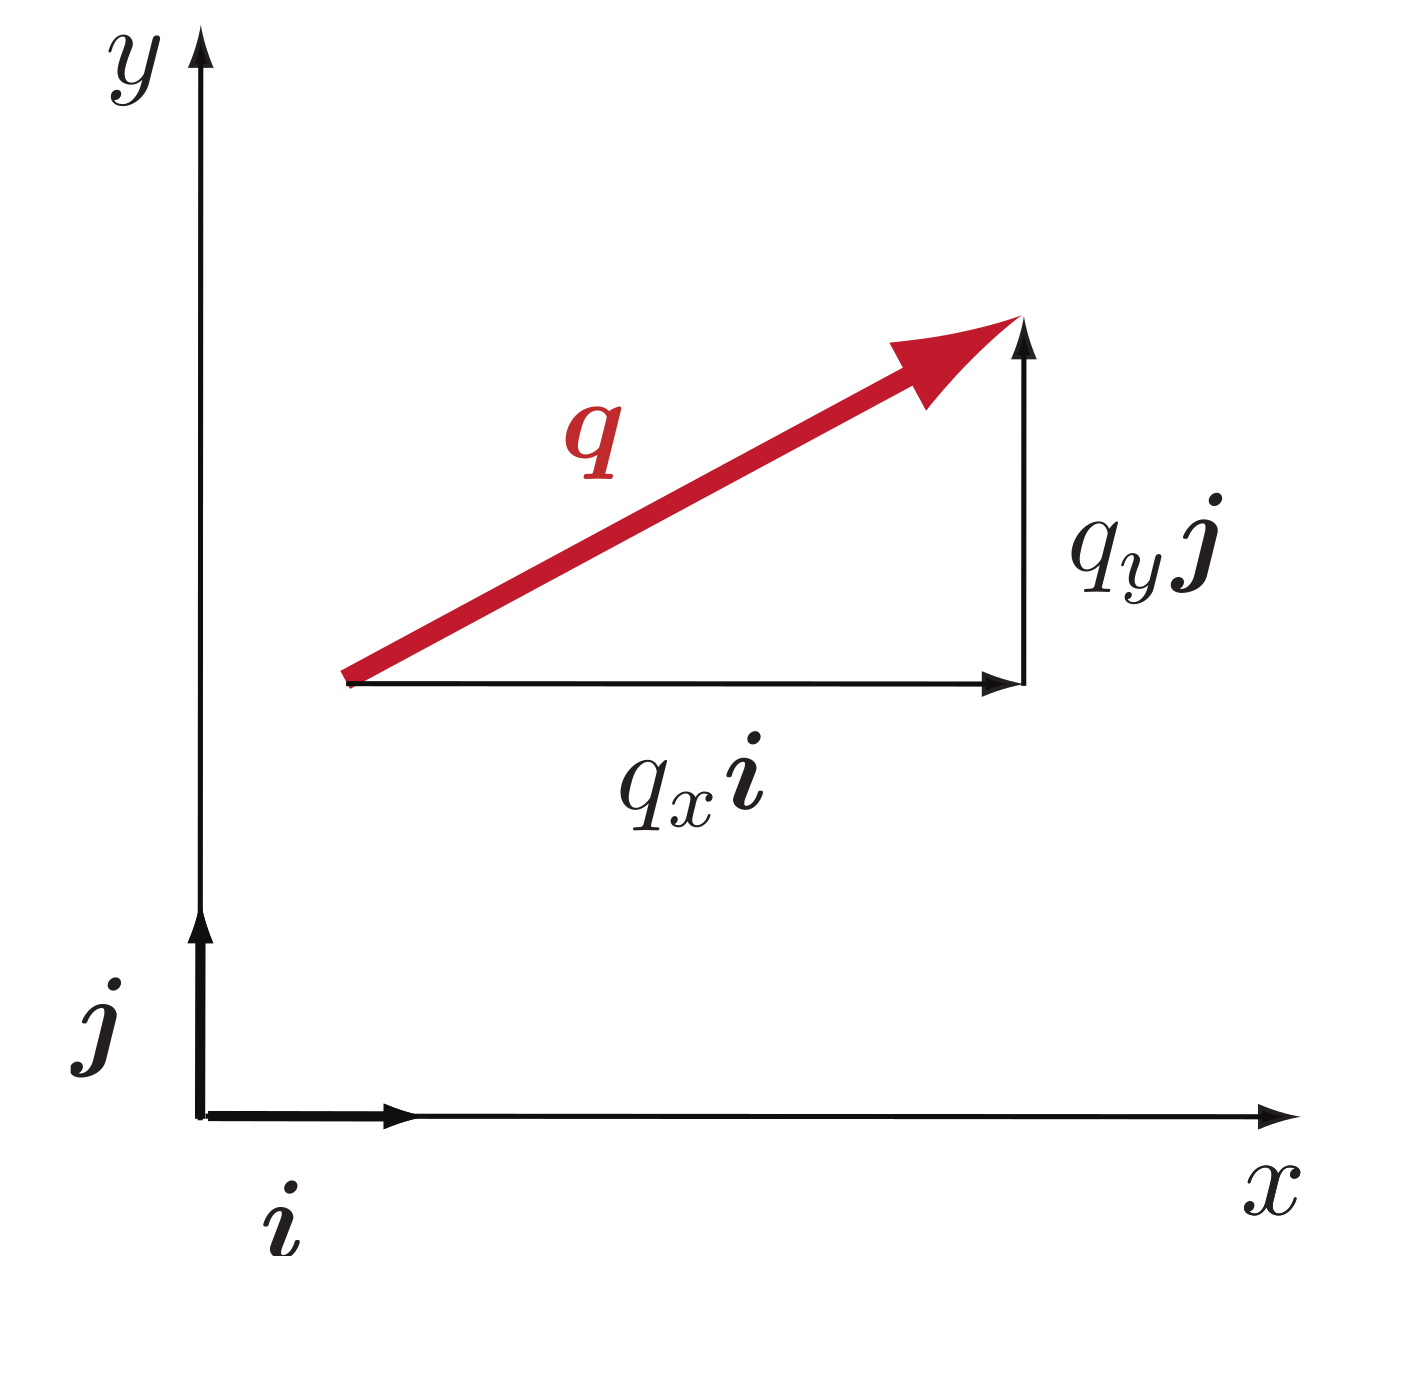
\includegraphics[width=0.25\textwidth]{figs/vector-q.png}
	\end{figure}
	\begin{equation*}
	\mathbf{q} = q_x \mathbf{i} + q_y \mathbf{j}
	\end{equation*}
	where $q_x$ is the $x-$component and $q_y$ is the $y-$component and $i$ and $j$ are basis vectors (are unit length).
	
	\textbf{Scalar product:}
	\begin{equation*}
	\mathbf{q} \cdot \mathbf{r} = \mathbf{q}^T \mathbf{r} = \begin{bmatrix} q_x & q_y \end{bmatrix} \begin{bmatrix} r_x \\ r_y \end{bmatrix} = q_x r_x + q_y r_y
	\end{equation*}
\end{frame}
%----------------------------------------------------------------------------------------
\begin{frame}
	\frametitle{Vector calculus}
	
	
	\textbf{Grad:} If the del operator acts on a scalar field, say temperature $T(x, y)$, it produces a vector
	that points in the direction of the steepest slope.
	
	\begin{equation*}
	\nabla \mathbf{T} =  
	\begin{bmatrix} 
	\frac{\partial T}{\partial x} \\
	\frac{\partial T}{\partial y}
	\end{bmatrix}
	\end{equation*}
	
	\textbf{Divergence:} The scalar product of the del operator with a vector field q gives the divergence
	\begin{equation*}
	div \mathbf{q} = \nabla \cdot \mathbf{q} = \frac{\partial q_x}{\partial x} + \frac{\partial q_y}{\partial y}
	\end{equation*}
	Notice the divergence of a vector field is a scalar.
	
	\textbf{Divergence theorem}
	\begin{equation*}
	\int_\Omega div \mathbf{q} d\Omega = \oint_\Gamma \mathbf{q}\cdot \mathbf{n} d\Gamma
	\end{equation*}
\end{frame}

\note{ 
	Divergence is the volume density of the outward flux.
	
	Gauss's theorem or Divergence theorem is a result that relates the flow (that is, flux) of a vector field through a surface to the behavior of the tensor field inside the surface.}

%----------------------------------------------------------------------------------------
\begin{frame}
	\frametitle{Vector calculus}
	\begin{figure}
		\centering
		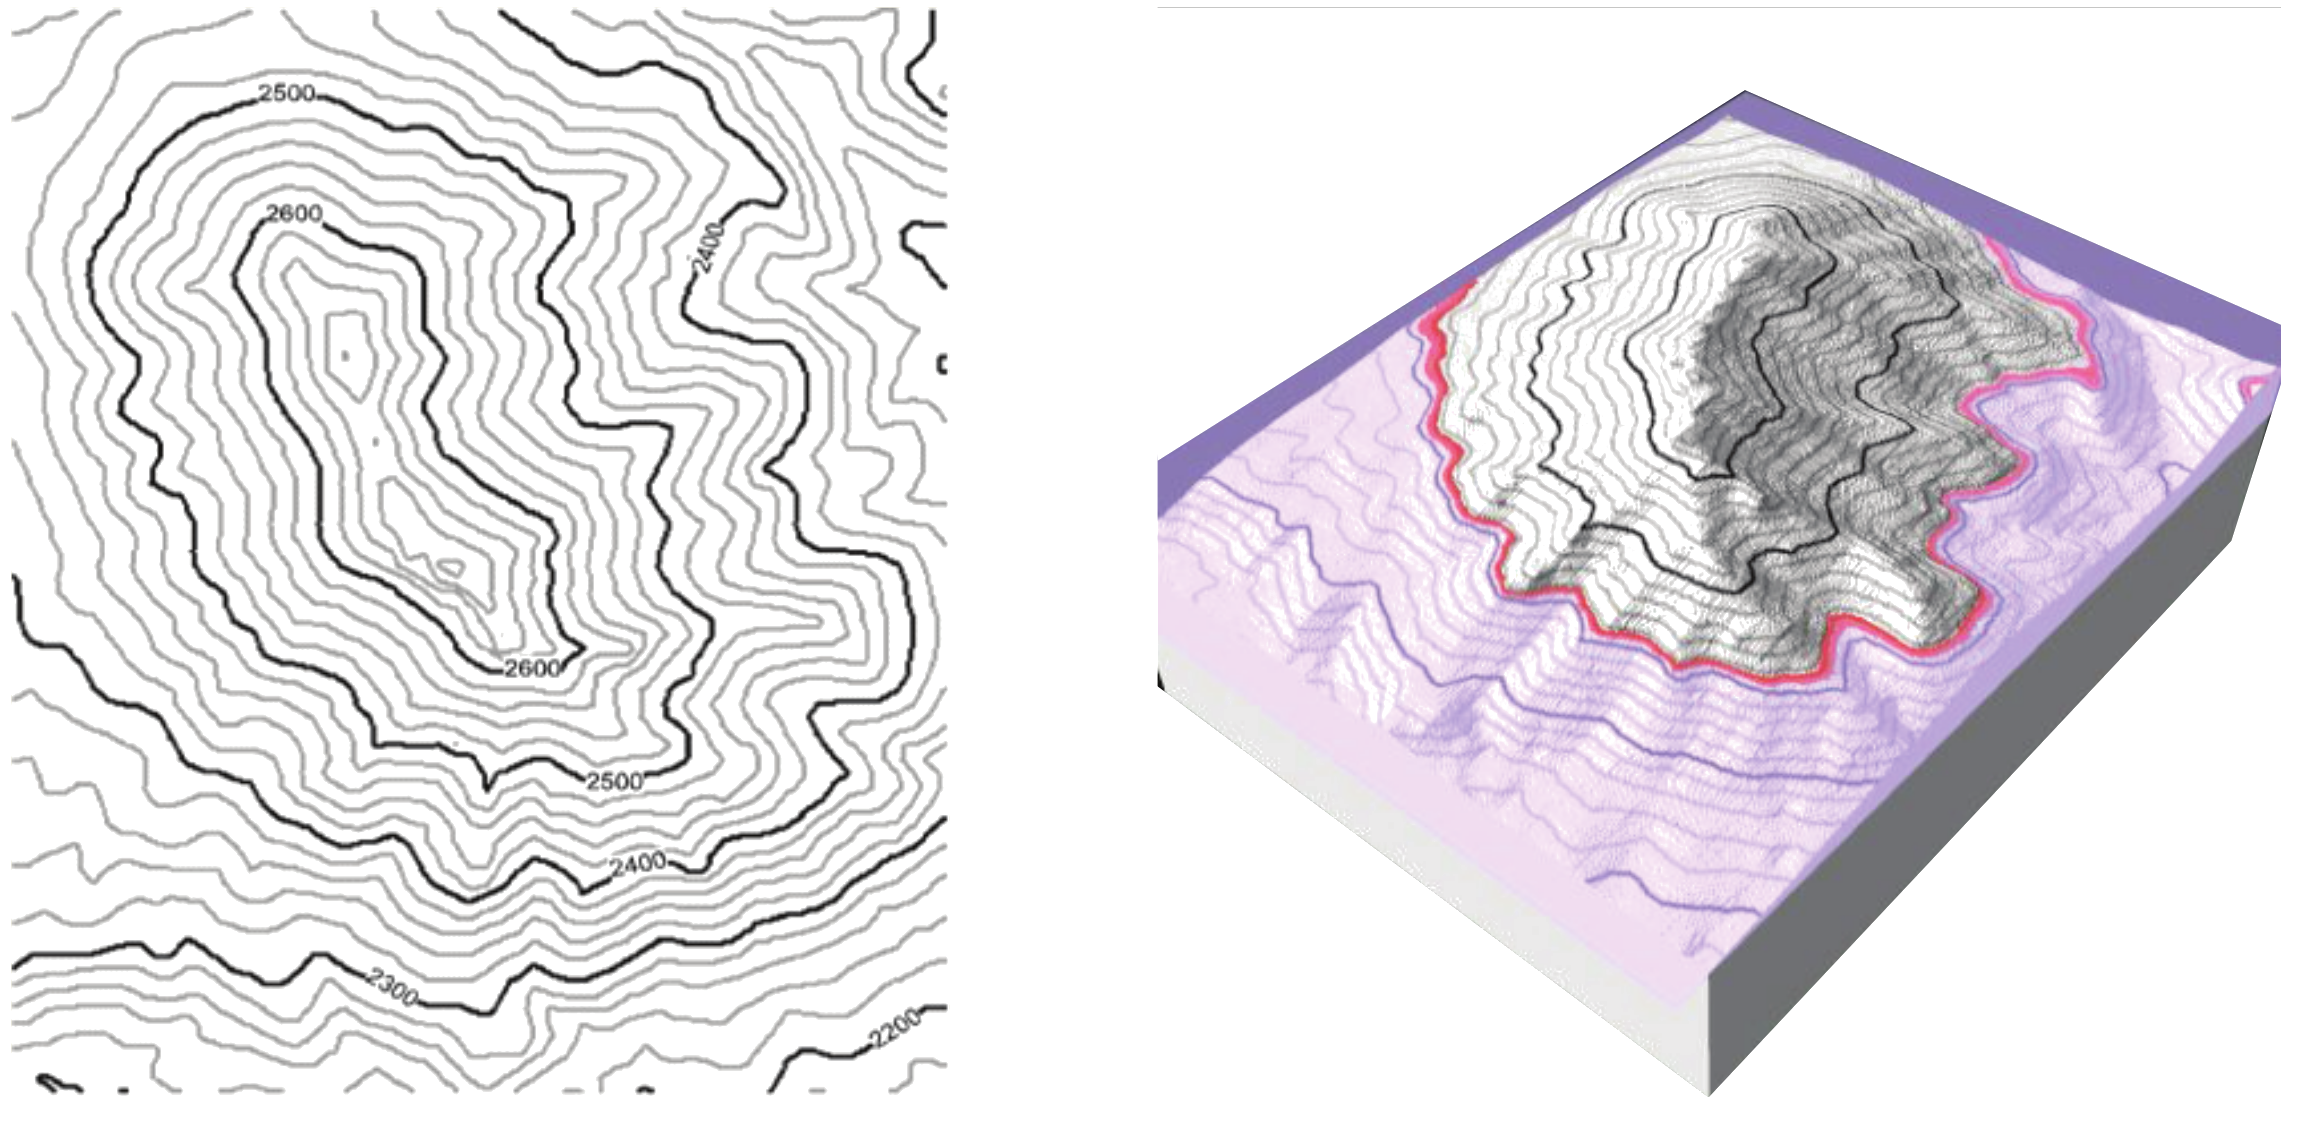
\includegraphics[width=\textwidth]{figs/grad-vector.png}
		\caption*{Contour map for a terrain (left) and the associated three-dimensional model (right). If $T$
			is interpreted as the height, the vector $\Delta T$ points in the direction of the steepest slope.}
	\end{figure}
\end{frame}

%----------------------------------------------------------------------------------------
\subsection{Index notation}
%----------------------------------------------------------------------------------------
\begin{frame}
	\frametitle{The summation convention}
	Suppose $\mathbf{x}$ and $\mathbf{y}$ are vectors, and \textbf{A} and \textbf{B} are matrices. Write a few common combinations in terms of their components:
	
	\begin{itemize}
		\item \textbf{Dot product: }
		\mode<beamer>{
			\begin{equation*}
			\mathbf{x}\cdot\mathbf{y} = \sum_{i = 1}^{n =3} x_i y_i
			\end{equation*}
		}  
		\mode<handout>{
			\vspace{1.5cm}
		} 
		\item \textbf{Matrix-vector product:} 
		\mode<beamer>{
			\begin{equation*}
			\left[\mathbf{Ax}\right]_i= \sum_{j = 1}^{n} A_{ij}x_j
			\end{equation*}
		}  
		\mode<handout>{
			\vspace{1.5cm}
		}
		\item \textbf{Matrix-vector product:} 	
		\mode<beamer>{
			\begin{equation*}
			\left[\mathbf{AB}\right]_{ij}= \sum_{k = 1}^{n} A_{ik}B_{kj}
			\end{equation*}
		}  
		\mode<handout>{
			\vspace{1.5cm}
		} 
	\end{itemize}
	
	\mode<beamer>{
		Every sum goes with an index which is repeated twice. Non-repeated indices are not summed.
	}  
	\mode<handout>{
		\vspace{1.5cm}
	} 
\end{frame}

%----------------------------------------------------------------------------------------
\begin{frame}
	\frametitle{The summation convention}
	We can use a simplified notation by adopting the summation convention (due to Einstein),
	Do not write the summation symbol $\sum$. A repeated index implies summation. (An index may not appear more than twice on one side of an
	equality.) Using the summation convention
	\begin{itemize}
		\item \textbf{Dot product: }
		\mode<beamer>{
			\begin{equation*}
			\mathbf{x}\cdot\mathbf{y} = x_i y_i
			\end{equation*}
		}  
		\mode<handout>{
			\vspace{1cm}
		} 
		\item \textbf{Matrix-vector product:} 
		\mode<beamer>{
			\begin{equation*}
			\left[\mathbf{Ax}\right]_i= A_{ij}x_j
			\end{equation*}
		}  
		\mode<handout>{
			\vspace{1cm}
		}
		\item \textbf{Matrix-vector product:} 	
		\mode<beamer>{
			\begin{equation*}
			\left[\mathbf{AB}\right]_{ij}= A_{ik}B_{kj}
			\end{equation*}
		}  
		\mode<handout>{
			\vspace{1cm}
		} 
	\end{itemize}
	This may seem a very peculiar trick, with no obvious benefit. However, it will turn out
	to be surprisingly powerful, and make many calculations involving vector identities and
	vector differential identities much simpler.
\end{frame}

%----------------------------------------------------------------------------------------
\begin{frame}
	\frametitle{The Kronecker delta $\delta_{ij}$}
	The identity matrix:
	\begin{equation*}
	\mathbf{I} = 
	\begin{bmatrix}
	1 & 0 & 0 \\
	0 & 1 & 0 \\
	0 & 0 & 1 \\
	\end{bmatrix}
	\end{equation*}
	
	We define the `\textit{Kronecker delta}' as:
	\mode<beamer>{
		\begin{equation*}
		\delta_{ij} = 
		\begin{cases}
		1 \quad i = j,\\
		0 \quad i \ne j
		\end{cases}
		\end{equation*}
	}  
	\mode<handout>{
		\vspace{1.5cm}
	} 
	
	We know that: $\mathbf{Iy} = \mathbf{y}$
	
	\mode<beamer>{
		\begin{equation*}
		\delta_{ij}y_j = y_i
		\end{equation*}
	}  
	\mode<handout>{
		\vspace{1.5cm}
	}
	In other words ‘if one index of $\delta_{ij}$ is summed, the effect is to swap this to the other
	index’.
\end{frame}


%----------------------------------------------------------------------------------------
\begin{frame}
	\frametitle{The permutation symbol $\epsilon_{ijk}$}
	Cross product of two vectors:
	\begin{equation*}
	\mathbf{x \times y} = 
	\begin{vmatrix}
	\mathbf{e}_1 & \mathbf{e}_2 & \mathbf{e}_1 \\
	x_1 & x_2 & x_3 \\
	y_1 & y_2 & y_3 \\
	\end{vmatrix} = 
	\begin{bmatrix}
	x_2 y_3 - x_3 y_2, & x_3 y_1 - x_1 y_3, &
	x_1 y_2 - x_2 y_1
	\end{bmatrix}
	\end{equation*}
	
	where $e_i$ are the basis for the vectors. We have assumed that $e_i$ are the unit vectors for
	Cartesian coordinates (you may have seen the basis vectors written as \textit{i}, \textit{j} and \textit{k}). To express the cross product in index notation, we will use the permutation symbol $\epsilon_{ijk}$. The permutation symbol $\epsilon_{ijk}$ is defined as:
	\mode<beamer>{
		\begin{equation*}
		\epsilon_{ijk} = 
		\begin{cases}
		1 \quad \text{if (\textit{ijk}) is an even permutation of (1, 2, 3)},\\
		-1 \quad \text{if (\textit{ijk}) is an odd permutation of (1, 2, 3)},\\
		0 \quad \text{otherwise}
		\end{cases}
		\end{equation*}
	}  
	\mode<handout>{
		\vspace{1.5cm}
	} 
\end{frame}


%----------------------------------------------------------------------------------------
\begin{frame}
	\frametitle{The permutation symbol $\epsilon_{ijk}$}
	For example:
	\mode<beamer>{
		\begin{align*}
		\epsilon_{112} = 0 \\
		\epsilon_{312} = 1 \\
		\epsilon_{132} = -1 \\		
		\end{align*}
	}  
	\mode<handout>{
		\vspace{1.5cm}
	} 
	The permutation symbol is also known as the ‘alternating symbol’ or the ‘Levi-Civita
	symbol’. Using the permutation symbol, we can write the cross product of two vectors as:
	\mode<beamer>{
		\begin{equation*}
		\left[\mathbf{x \times y}\right] = \epsilon_{ijk} x_j y_k
		\end{equation*}
		To prove this, for each \textit{i} sum over \textit{j} and \textit{k}. The permutation symbol possesses a number of ‘symmetries’,
		\begin{align*}
		&\epsilon_{ijk} = \epsilon_{kij} = \epsilon_{jki} \text{ (cyclic permutation)}\\
		&= -\epsilon_{jik} = -\epsilon_{ikj} = -\epsilon_{kji} \text{ (switch pair \textit{ij}, switch pair \textit{ki}, switch pair \textit{jk})}\\
		\end{align*}
	}  
	\mode<handout>{
		\vspace{3.5cm}
	} 
\end{frame}


%----------------------------------------------------------------------------------------
\begin{frame}
	\frametitle{Vector derivatives}
	The real power of index notation is revealed when we look at vector differential identities.
	The vector derivatives known as the gradient, the divergence and the curl can all be
	written in terms of the operator $\nabla$
	\begin{equation*}
	\nabla = \begin{bmatrix}
	\frac{\partial}{\partial x_1}, &
	\frac{\partial}{\partial x_2}, &
	\frac{\partial}{\partial x_3}
	\end{bmatrix}
	\end{equation*}
	where $\left[x_1, x_2, x_3 \right]$ are the components of the position vector $\mathbf{x}$.
	\begin{itemize}
		\item \textbf{Gradient:}
		\mode<beamer>{
			\begin{equation*}
			grad \phi: [\nabla \phi]_i = \frac{\partial \phi}{\partial x_i} = \begin{bmatrix}
			\frac{\partial \phi}{\partial x_1}, &
			\frac{\partial \phi}{\partial x_2}, &
			\frac{\partial \phi}{\partial x_3}
			\end{bmatrix}
			\end{equation*}
		}  
		\mode<handout>{
			\vspace{1cm}
		} 
		\item \textbf{Divergence:} 
		\mode<beamer>{
			\begin{equation*}
			div \mathbf{u}: \nabla \cdot \mathbf{u}  = \frac{\partial u_i}{\partial x_i} = 
			\frac{\partial u_1}{\partial x_1} +
			\frac{\partial u_2}{\partial x_2} +
			\frac{\partial u_3}{\partial x_3}	
			\end{equation*}
		}  
		\mode<handout>{
			\vspace{1cm}
		}
		\item \textbf{Curl: $[\mathbf{a \times b}]_i = \epsilon_{ijk} a_j b_k$} 	
		\mode<beamer>{
			\begin{equation*}
			curl \mathbf{u}: \left[\nabla \times \mathbf{u}\right]_i = \epsilon_{ijk}\frac{\partial u_k}{\partial x_j}
			\end{equation*}
		}  
		\mode<handout>{
			\vspace{1cm}
		} 
	\end{itemize}
\end{frame}


%----------------------------------------------------------------------------------------
\begin{frame}
	\frametitle{Cauchy stress tensor}
	To establish the relationship between $\mathbf{t}$ and $\mathbf{\hat{n}}$ we now set up an infinitesimal
	tetrahedron in Cartesian coordinates:
	\begin{figure}[ht]
		\centering
		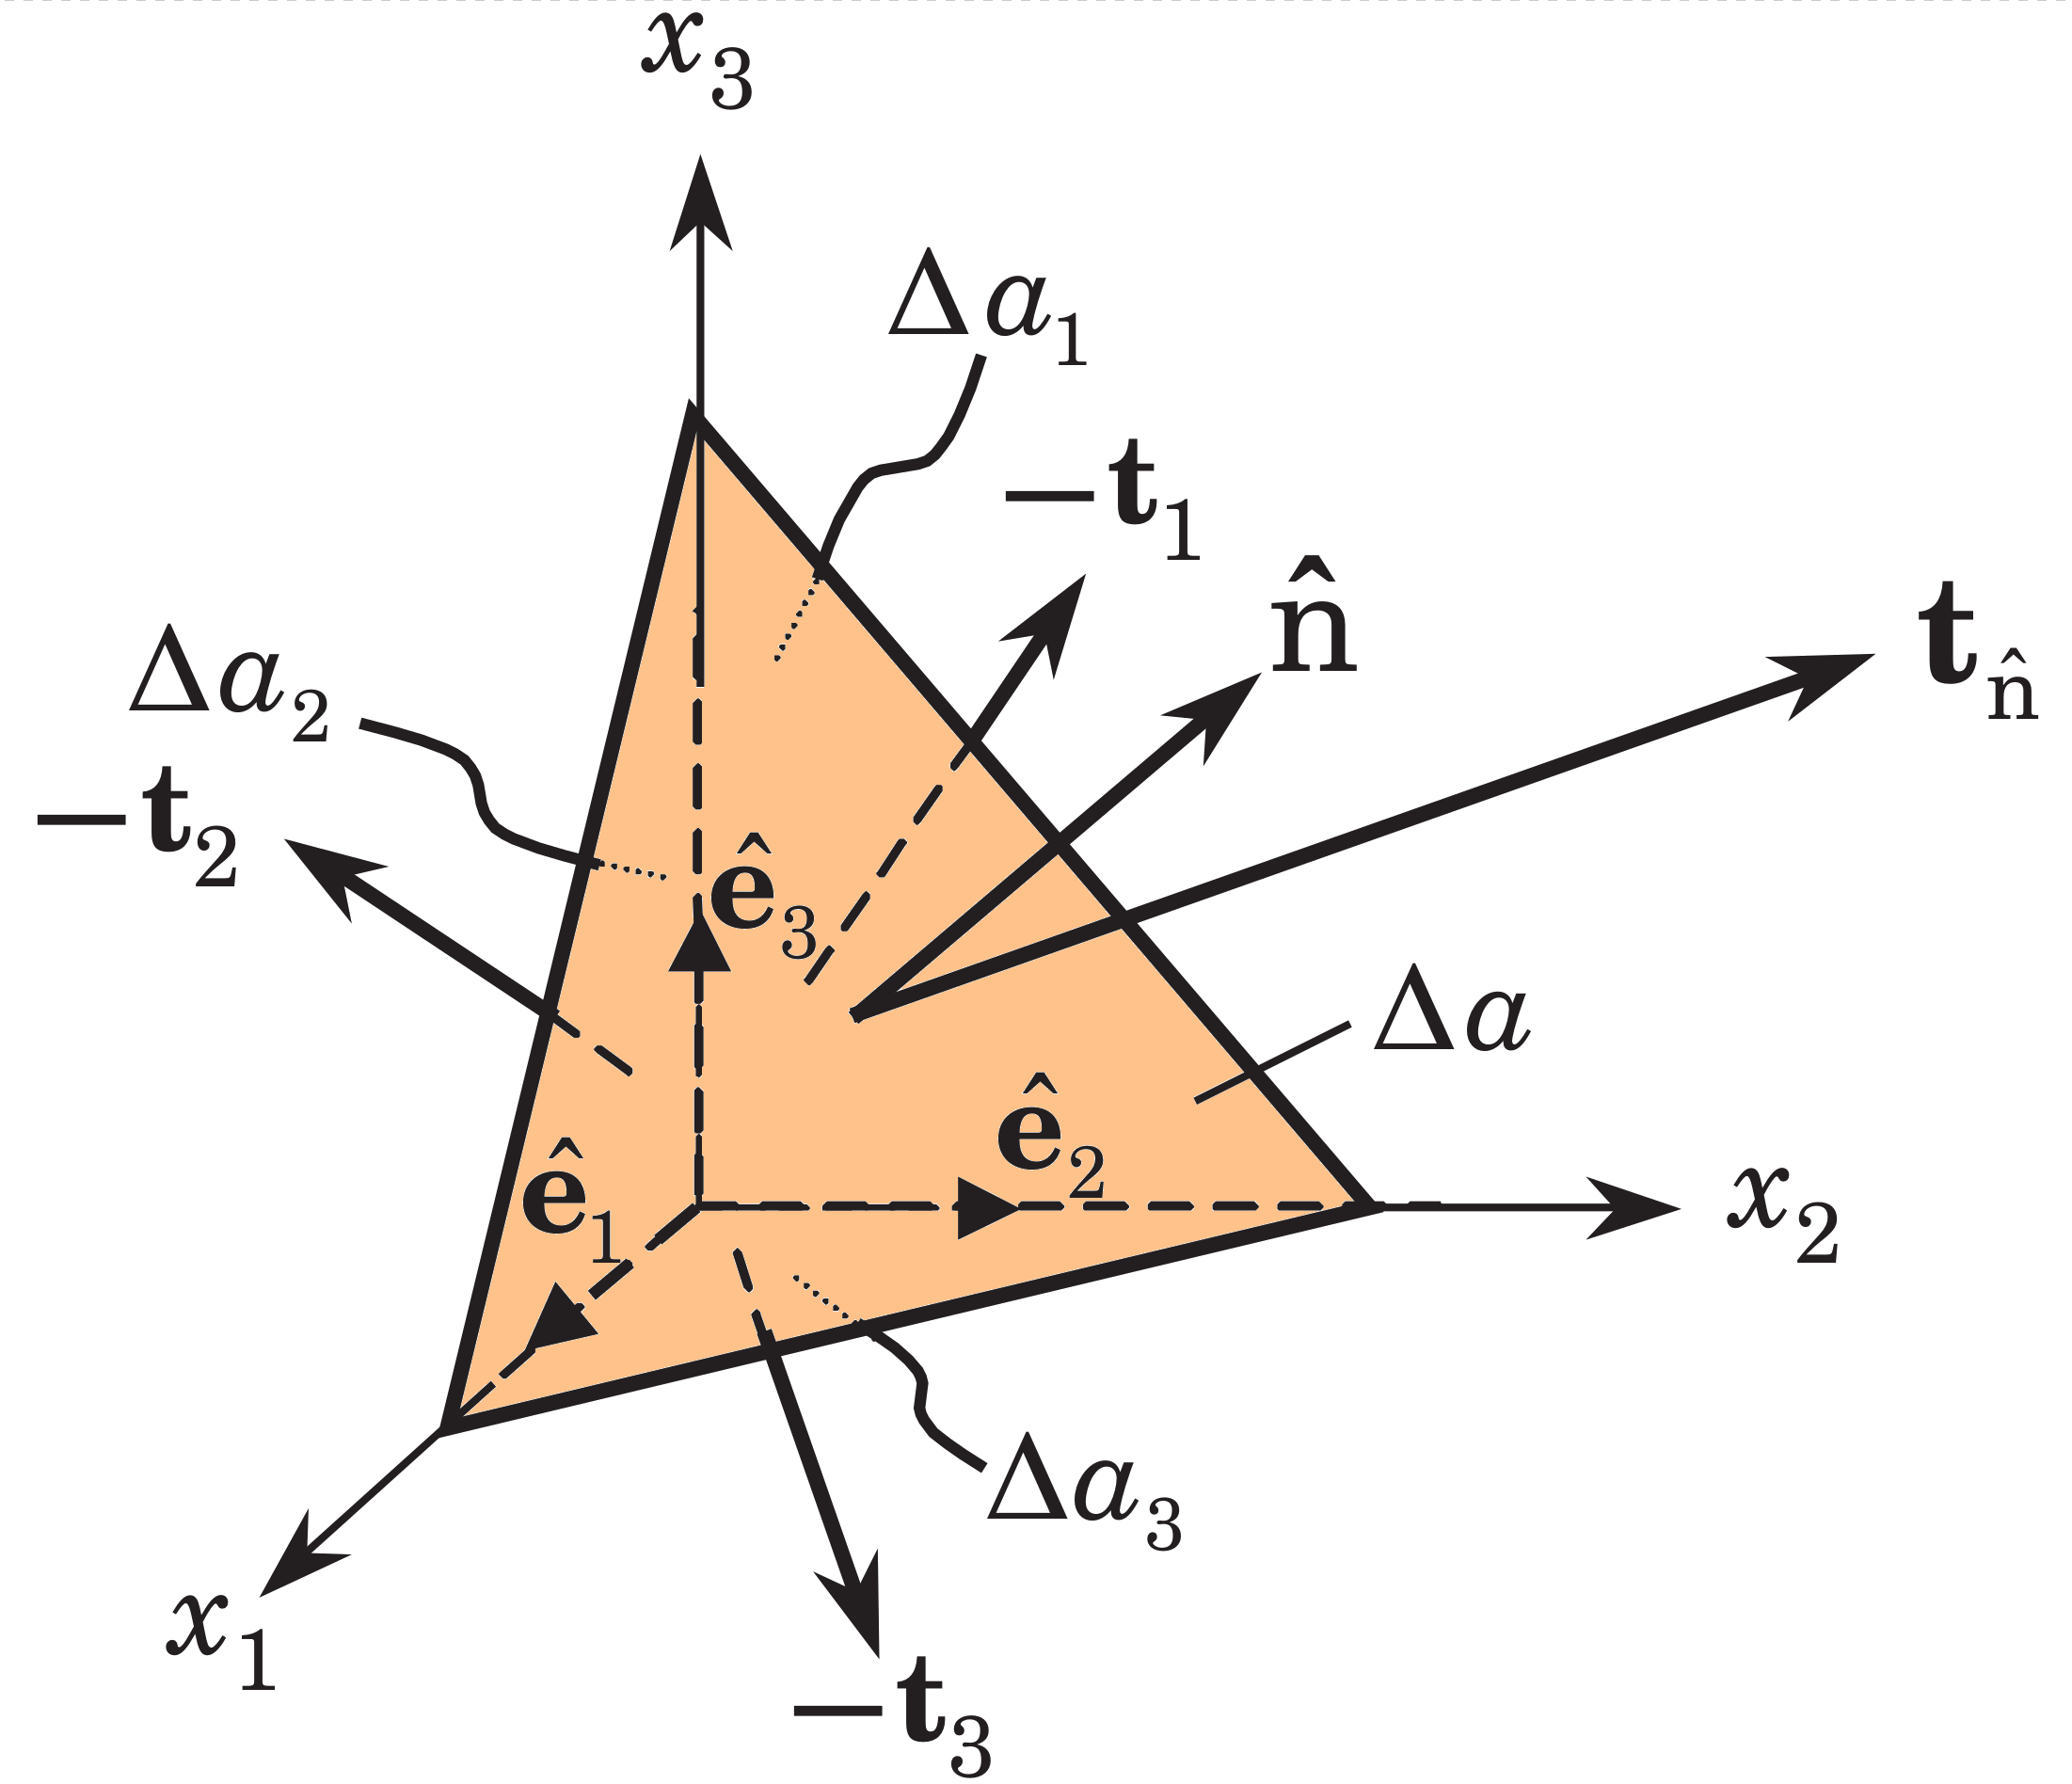
\includegraphics[width=0.4\textwidth]{figs/stress-tetrahedron.png}
		%\caption*{Tetrahedral element in Cartesian coordinates (Reddy., 2008)}
	\end{figure}
	If $\mathbf{-t}_1, \mathbf{-t}_2, \mathbf{-t}_3$ and $\mathbf{t}$ denote the stress vectors in the outward directions on the faces of the infinitesimal tetrahedron whose areas are $\Delta a_1, \Delta a_2, \Delta a_3$, and $\Delta a$, respectively. $\Delta v$ is the volume of the tetrahedron, $\rho$ the density, $f$ the body force per unit mass, and $\mathbf{a}$ the acceleration. 
\end{frame}

%----------------------------------------------------------------------------------------
\begin{frame}
	\frametitle{Cauchy stress tensor}
	we have by Newton's second law for the mass inside the tetrahedron:
	\mode<beamer>{	
		\begin{equation*}
		\mathbf{t}\Delta a - \mathbf{t}_1 \Delta a_1
		- \mathbf{t}_2 \Delta a_2 - \mathbf{t}_3 \Delta a_3 + \rho \Delta v \mathbf{f} = \rho \Delta v \mathbf{a}
		\end{equation*}
	}
	\mode<handout>{
		\vspace{1.5cm}
	}
	
	Since the total vector area of a closed surface is zero (gradient theorem):
	\mode<beamer>{	
		\begin{equation*}
		\Delta a \mathbf{\hat{n}} - \Delta a_1 \mathbf{\hat{e}}_1 - \Delta a_2 \mathbf{\hat{e}}_2
		- \Delta a_3 \mathbf{\hat{e}}_3 = \mathbf{0}
		\end{equation*}
		\begin{equation*}
		\Delta a_1 =
		(\mathbf{\hat{n}}\cdot\mathbf{\hat{e}}_1) \Delta a, \quad 
		\Delta a_2 = (\mathbf{\hat{n}}\cdot\mathbf{\hat{e}}_2) \Delta a, \quad 
		\Delta a_3 = (\mathbf{\hat{n}}\cdot\mathbf{\hat{e}}_3) \Delta a. 
		\end{equation*}
	}
	\mode<handout>{
		\vspace{1.5cm}
	}
	
	The volume $\Delta v$ can be expressed as: \mode<beamer>{$\Delta v = (\Delta h / 3) \Delta a$}
	where $\Delta h$ is the perpendicular distance from the origin to the slant face.
	\mode<beamer>{	
		\begin{equation*}
		\mathbf{t} = 
		(\mathbf{\hat{n}}\cdot\mathbf{\hat{e}}_1) \mathbf{t}_1 +
		(\mathbf{\hat{n}}\cdot\mathbf{\hat{e}}_2) \mathbf{t}_2 + 
		(\mathbf{\hat{n}}\cdot\mathbf{\hat{e}}_3) \mathbf{t}_3 + \rho \frac{\Delta h}{3}(\mathbf{a - f})
		\end{equation*}
	}
	\mode<handout>{
		\vspace{1.5cm}
	}
\end{frame}

%----------------------------------------------------------------------------------------
\begin{frame}
	\frametitle{Cauchy stress tensor}
	In the limit when the tetrahedron shrinks to a point $\Delta h \to 0$:
	\begin{equation*}
	\mathbf{t} = 
	(\mathbf{\hat{n}}\cdot\mathbf{\hat{e}}_1) \mathbf{t}_1 +
	(\mathbf{\hat{n}}\cdot\mathbf{\hat{e}}_2) \mathbf{t}_2 + 
	(\mathbf{\hat{n}}\cdot\mathbf{\hat{e}}_3) \mathbf{t}_3 = (\mathbf{\hat{n}}\cdot\mathbf{\hat{e}}_i) \mathbf{t}_i
	\end{equation*}
	where the summation convention is used.
	\mode<beamer>{	
		\begin{equation*}
		\mathbf{t} = 
		\mathbf{\hat{n}}\cdot(\mathbf{\hat{e}}_1 \mathbf{t}_1 +
		\cdot\mathbf{\hat{e}}_2 \mathbf{t}_2 + 
		\mathbf{\hat{e}}_3 \mathbf{t}_3).
		\end{equation*}
	}
	\mode<handout>{
		\vspace{1.5cm}
	}
	
	The terms in the parenthesis is the 
	\textit{\textbf{stress tensor}} $\sigma$:
	\begin{equation*}
	\sigma \equiv \mathbf{\hat{e}}_1 \mathbf{t}_1 +
	\cdot\mathbf{\hat{e}}_2 \mathbf{t}_2 + 
	\mathbf{\hat{e}}_3 \mathbf{t}_3
	\end{equation*}
	The stress tensor is a property of the medium that is independent of the $\mathbf{\hat{n}}$
	\mode<beamer>{	
		\begin{equation*}
		\mathbf{t}(\mathbf{\hat{n}}) = 
		\mathbf{\hat{n}} \cdot \sigma = \sigma^T \mathbf{\hat{n}}
		\end{equation*}
	}
	\mode<handout>{
		\vspace{1.5cm}
	}
	The stress vector $\mathbf{t}$ represents the vectorial stress on a plane whose normal is $\mathbf{\hat{n}}$. $\sigma$ is the \textit{Cauchy stress tensor} defined to be the \textit{current force per unit deformed area}. In Cartesian component, the Cauchy formula is: $t_i = n_j \sigma_{ji}$.
\end{frame}


%----------------------------------------------------------------------------------------
\begin{frame}
	\frametitle{Cauchy stress vs Piola-Kirchoff stress}
	\begin{figure}[ht]
		\centering
		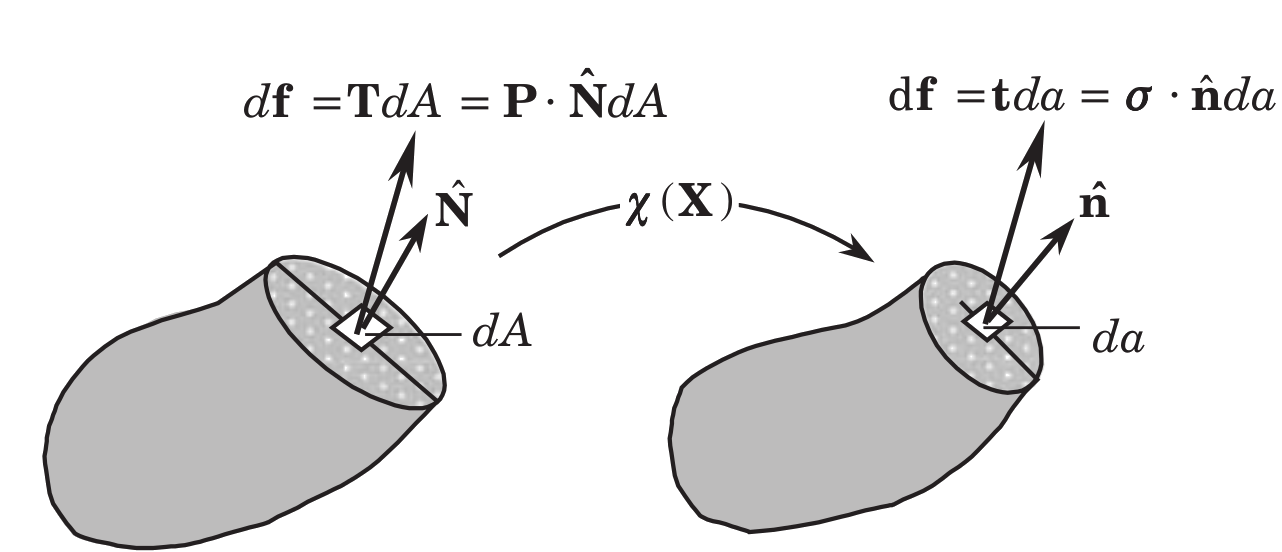
\includegraphics[width=\textwidth]{figs/cauchy-kirchoff-stress-tensor.png}
		\caption*{An introduction to continuum mechanics - J. N. Reddy (2008)}
	\end{figure}
	\mode<beamer>{
		\begin{itemize}
			\item The first Piola–Kirchhoff stress tensor, also referred to as the \textit{nominal stress tensor},
			or \textit{Lagrangian stress tensor}, gives the current force per unit undeformed area.
		\end{itemize}
	}
	\mode<handout>{
		\vspace{2cm}
	}
\end{frame}

\subsection{Displacement fields}

\note{
	For a given geometry and loading, the body \textit{B} will undergo macroscopic geometric
	changes within the body, which are termed deformation. The geometric changes are
	accompanied by stresses that are induced in the body.
	In the Lagrangian description, the displacements are expressed in terms of the 
	material coordinates $X_i$: $\mathbf{u}(\mathbf{X}, t) = \mathbf{x}(\mathbf{X}, t) - \mathbf{X}$.
}


%----------------------------------------------------------------------------------------
\begin{frame}
	\frametitle{Displacement field}
	Consider 1D mapping $\mathbf{x} = \mathbf{X}(1 + 0.5t)$ defining the motion of a rod of initial
	length two units. The rod experiences a temperature distribution $T$ given by the
	material description $T = 2\mathbf{X}t^2$ or by the spatial description $T = 2\mathbf{x}t^2 /(1 + 0.5t)$
	\begin{figure}
		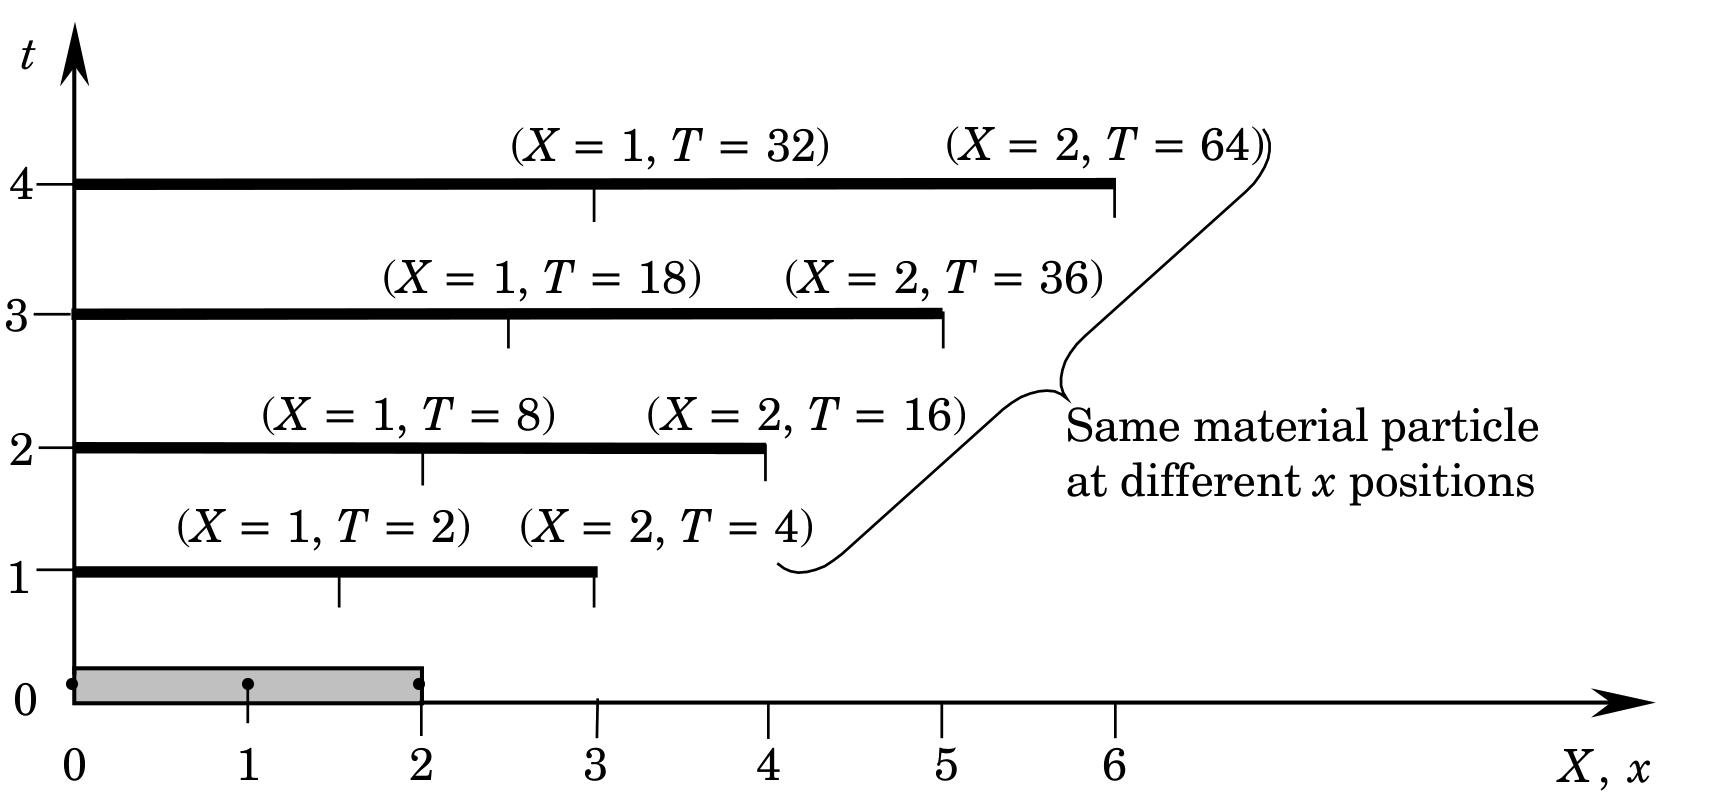
\includegraphics[width=0.85\textwidth]{figs/eulerian-lagrangian.png}
		\caption*{Material and spatial descriptions of motion (Reddy., 2008)}
	\end{figure}
\end{frame}

\note{
	From the figure, we see that the particle’s material coordinate (label) $X$
	remains associated with the particle while its spatial position $x$ changes. The
	temperature at a given time can be found in one of the two ways: for example,
	at time $t = 3$, the temperature of the particle labeled $X = 2$ is $T = 2 \times 2 \times (3)^2 = 36$;
	alternatively, the temperature of the same particle which at $t = 3$ is at a spatial position $x = 2(1 + 0.5 \times 3) = 5$ is $T = 2\times5(3)^2 /(1 + 0.5 \times 3) = 36$. The displacement
	of a material point occupying position $X$ in $k_0$ is:
	\begin{equation*}
	\mathbf{u}(\mathbf{X}, t) = \mathbf{x}(\mathbf{X}, t) - \mathbf{X} = X(1 + 0.5t) - X = 0.5Xt.
	\end{equation*}
}


%----------------------------------------------------------------------------------------
\begin{frame}
	\frametitle{Strains}
	
	\begin{figure}
		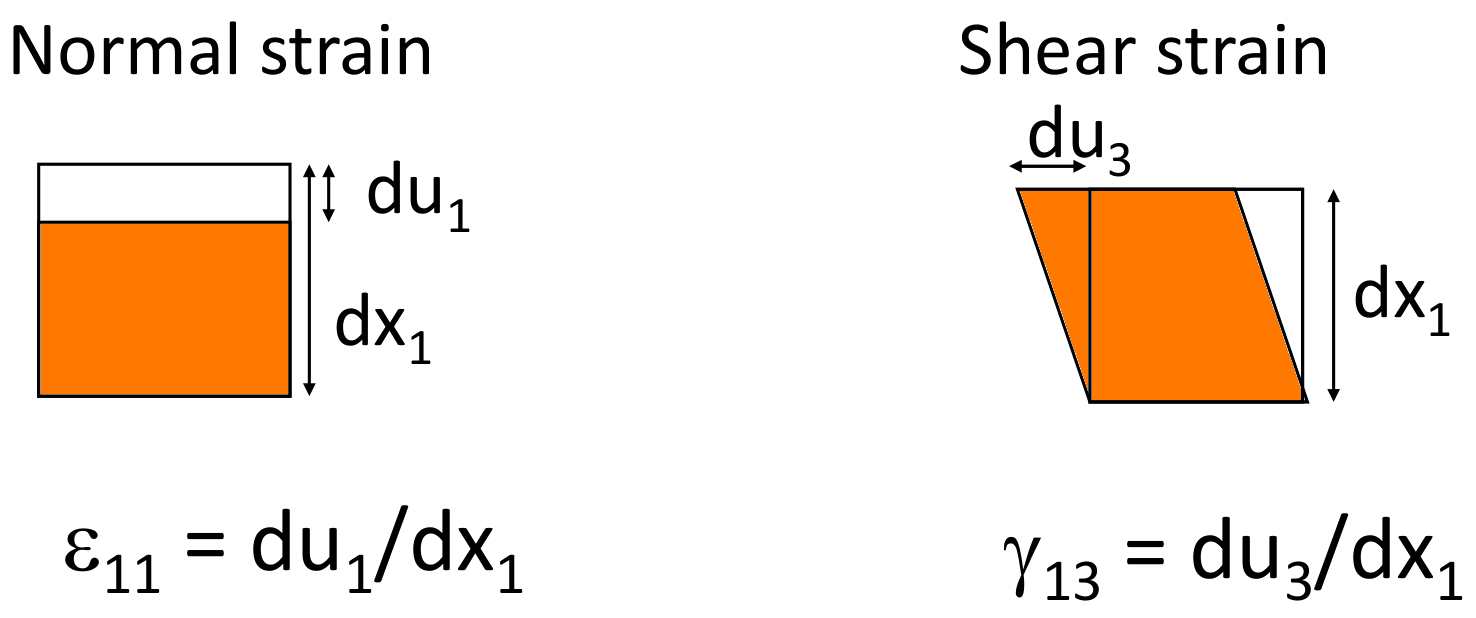
\includegraphics[width=\textwidth]{figs/strain.png}
	\end{figure}
	
	\mode<beamer>{	
		\begin{itemize}
			\item 6 strains: $\varepsilon_{11}, \varepsilon_{22}, \varepsilon_{33}, \gamma_{12}, \gamma_{23}, \gamma_{31}$.
			\item $\gamma_{21} = -\gamma_{12}, \gamma_{32} = - \gamma_{23}, \gamma_{13} = - \gamma_{31}$
			\item Compression is positive
			\item anti-clockwise is positive
		\end{itemize}
	}
\end{frame}

\end{document}
